\documentclass{article}

\usepackage{PRIMEarxiv}

\usepackage[utf8]{inputenc} % allow utf-8 input
\usepackage[T1]{fontenc}    % use 8-bit T1 fonts
\usepackage{hyperref}       % hyperlinks
\usepackage{url}            % simple URL typesetting
\usepackage{booktabs}       % professional-quality tables
\usepackage{amsfonts,amsmath}       % blackboard math symbols
\usepackage{nicefrac}       % compact symbols for 1/2, etc.
\usepackage{microtype}      % microtypography
\usepackage{lipsum}
\usepackage{fancyhdr}       % header
\usepackage{graphicx}       % graphics
\usepackage{subcaption}
\usepackage{transparent}
\usepackage{color}
\graphicspath{{media/}}     % organize your images and other figures under media/ folder
\renewcommand{\baselinestretch}{1.5} 

%Header
\pagestyle{fancy}
\thispagestyle{empty}
\rhead{ \textit{ }} 
% Update your Headers here
\fancyhead[LO]{Far-field potential flow conditions for Immersed Cartesian meshes}
% \fancyhead[RE]{Firstauthor and Secondauthor} % Firstauthor et al. if more than 2 - must use \documentclass[twoside]{article}



  
%% Title
\title{Simulations of unbounded external flows on using minimal Eulerian grids
%%%% Cite as
%%%% Update your official citation here when published 
\thanks{\textit{\underline{Citation}}: 
\textbf{Authors. Title. Pages.... DOI:000000/11111.}} 
}

\author{
    Gabriel D. Weymouth\\
    Faculty of Mechanical Engineering (mE) \\
    Delft University of Technology, Delft, Netherlands \\
    \texttt{G.D.Weymouth@tudelft.nl} \\
    \AND
    Marin Lauber\\
    Faculty of Mechanical Engineering (mE) \\
    Delft University of Technology, Delft, Netherlands \\
    \texttt{M.Lauber@tudelft.nl} \\
  %% \AND
  %% Coauthor \\
  %% Affiliation \\
  %% Address \\
  %% \texttt{email} \\
  %% \And
  %% Coauthor \\
  %% Affiliation \\
  %% Address \\
  %% \texttt{email} \\
  %% \And
  %% Coauthor \\
  %% Affiliation \\
  %% Address \\
  %% \texttt{email} \\
}


\begin{document}
\maketitle


\begin{abstract}
We introduce a novel boundary condition formulation for external flow simulations on Eulerian grids that maintains high accuracy results even when the domain boundary is close to the immersed solid boundaries. The boundary condition is formulated using a \emph{Biot-Savart} vorticity integral inside the fluid domain along with the incompressible and irrotational flow conditions outside the domain. These conditions are incorporated in a general projection-based fluid flow solver using the standard velocity-pressure Eulerian fields. We use a multilevel approach to reduce the computational cost of the evaluation of the \emph{Biot-Savart} integral from $O(N^2)$ to $O(N\log N)$ and formally bound the associated error. We demonstrate the ability of the method to correctly impose far-field with multiple examples of vortex formation flows and drag and thrust wakes,  potential flow boundary conditions with domain size significantly smaller than when standard boundary conditions are used. Finally, we study the sensitivity of deflected wakes to the new domain boundary conditions. 
\end{abstract}


% keywords can be removed
\keywords{Biot-Savart \and Boundary Condition \and Projection Method \and Unbounded Domains}

\section{Introduction}
% introduce the problem
Numerical solutions to a continuum problem in an unbounded domain occur in numerous scientific fields, such as fluid mechanics, theoretical physics \cite{Levy2022SolvingMethod}, and electromagnetism \cite{}. To obtain a numerical solution to this continuum problem, common practice to introduce two approximations. First, the continuum is approximated by a discrete set of equations, and second, the unbounded domain is truncated to a much smaller computational domain. While the former does not usually introduce large errors, the latter can significantly impact the numerical solution to the continuum problem when this truncated domain is not \emph{sufficiently large}. In the context of computational fluid dynamics, \emph{sufficiently large} means that the decaying potential flow induced by the body (or equivalently, in immersed-boundary methods, the system of forces) and the advection/diffusion of vorticity through the domain's boundary have no influence on the forces experienced by the body \cite{Colonius2008}.

% introduce why we need far-field BCs
In numerical simulations of external incompressible flows, the problem we will focus on, \emph{far-field} boundary conditions, are applied on the (\emph{sufficiently large}) computational domain's exterior. These far-field boundary conditions consist of a known velocity normal to the boundary and a known normal pressure gradient (for a description of the boundary conditions for the incompressible \emph{Navier-Stokes} equations, we refer the reader to \cite{Gresho1987}). While they allow for a finite computational time, these lead to significant errors, particularly the force acting on a body can suffer from severe \emph{blockage effects} when the computational domain is not \emph{sufficiently large} \cite{Colonius2008}. While domain sensitivity study can determine the extent of the blockage effect, there is no \emph{a priori} rule for estimating these errors.

% what have people been doing
Numerous methods have been proposed to solve this issue for external incompressible flows and for unbounded continuum equations more generally. One method used to reduce the source of both these errors is to use rectilinear grid stretching to maximize the domain size and minimize the error at the far-field while maintaining a high-resolution uniform grid around the body, see \cite{Maertens2015, Lauber2022}. However, this method requires correct stretching ratios to avoid excessive numerical dissipation or reflection inside the domain. The method is also inefficient in cases where the body undergoes substantial motion within that domain, for example, when tracking the motion of a kite, which requires a sizeable uniform domain and an even larger stretched region. Grid stretching can also be replaced with buffer layer methods that apply a filter to the equations and mimic unbounded domains \cite{Colonius2002ADomains}, however, the method is limited to compressible flows, which are out of the scope of this paper.

% proposed to use a coordinate transform to effectively map the computational domain's boundary to infinity and apply the true boundary condition there. However, this approach is limited to trivial one-dimensional cases and cannot be extended to three-dimensional flow simulations. Similarly, methods where a limited number of dimensions are unbounded have been successfully proposed. 
While methods exist for incompressible flow problems unbounded in one \cite{Grosch1977NumericalTransforms, Levy2022SolvingMethod} or two directions \cite{Rennich1997NumericalDirections}, a method that enables accurate modeling of a flow unbounded in all directions still lacks. The approach ue in these methods is to either use coordinate transforms to map the unbounded domain onto the interval $[0,1]$, or use analytical potential flow solution in the unbounded directions based on the classical decomposition of the velocity field into
\begin{equation}
    \vec{u} = \vec{u}_\omega + \nabla\phi + \vec{U}_\infty = -\nabla^{-2}\left(\nabla \times \vec{\omega}\right) + \nabla\phi + \vec{U}_\infty
\end{equation}
where $\vec{u}_\omega$ is the vortical component, $\nabla\phi$ is the potential component and $\vec{U}_\infty$ is the free-stream velocity. Fourier-based methods can then be used to solve for the vortical and potential of the velocity field. Matching the internal and external solution and their derivatives on the domain's boundary closes the system, and the unbounded boundary condition is satisfied on the domain's exterior, at the cost of an augmented system of equations.

% The vortical component is computed by the Fourier solution to the Laplace equation, augmented to capture the zero-mode solution (mean vorticity)
% \begin{equation}\label{eq:u_vort}
%     \vec{u}_\omega = -\nabla^{-2}\left(\nabla \times \vec{\omega}\right).
% \end{equation}
% By solving the Laplace equation $\nabla^2\phi=0$ is cylindrical coordinates via Fourier expansions, the velocity potential can be expressed in terms of Bessel functions of the first and second kind. Matching the internal and external solution and their derivatives on the domain's boundary closes the system, and the unbounded boundary condition is satisfied on the domain's exterior at the cost of an augmented system of equation.

When analytical expression for the potential and vortical component cannot be obtained simply, a large coarse grid can provide boundary conditions to a relatively small, well-resolved domain. This is the basis of the multi-domain method proposed in \cite{Colonius2008}. The method places a small, well-resolved, around the immersed body and interpolates the coarse solution to the finer domain's wall, providing artificial far-field boundary conditions to the innermost domain (the finest). The method is attractive as the computational cost on the coarse domain can be significantly reduced. 

\cite{Liska2014AEquations} applied to incompressible flows with immersed-boundaries \cite{Liska2017AFunctions} \cite{Liska2016ADomains}

\cite{Tsynkov1998NumericalReview}


Other methods leverage the strength of an Eulerian-based solver for the near body and Lagrangian solvers for the far wake by coupling a near wall Eulerian solver to a Vortex particle method in the wake \cite{Billuart2023AFlows}. They enable tracking the coarser wake for an extended time while enabling accurate modeling of the developing boundary layer on the object's surface. However, several (user-defined) parameters are required to correctly interpolate the Vortex particle method solution onto the Eulerian mesh. Extension to three-dimensional flow is possible but will significantly increase the computational cost.

All these methods allow for a reduction of the error introduced by truncating an infinite computational domain. However, their generality is often limited to specific discretization of the governing equations or introduces complex coupling procedures.
 
In this manuscript, we propose a novel method for imposing external potential-flow boundary conditions on the velocity and pressure fields on the exterior of a Cartesian computational domain. The method retains the primitive variables formulation ($\vec u$ and $p$) of the covering equations and is compatible with immersed boundaries. Additionally, it does not introduce additional Lagrangian or Eulerian mesh. In the next section, we describe the \emph{Biot-Savart} boundary conditions and how they are injected into a projection algorithm to solve the \emph{Navier-Stokes} equations. Next, we demonstrate the accuracy of the velocity reconstruction and the balance between speedup and accuracy in the reconstructed field. We then demonstrate, with confined vorticity and vortex-street examples, that the new boundary conditions significantly outperform standard reflective boundary both in terms of computational time and solution accuracy. We present unexpected result that the new method continues to perform well when the fundamental assumption of potential flow external to the domain is violated, and use the unstable deflected wakes generated by fast flapping foils to study the limits of the approach. We close this manuscript with a discussion of the method's applicability to various flows in science and engineering.

% Immersed-boundary (IB) are a class of numerical methods to solve partial differential equations with immersed objects. The method relies on a Cartesian, static background grid and represents the immersed object or interface by a set of Lagrangian points \cite{Peskin2010}, analytical distance function \cite{Maertens2015}, or any other adequate representation. This class of method has been successfully applied to modeling the flow around moving boundaries or objects \cite{Mittal2005}. In this case, the viscous flow equations are solved on the background grid, and a volumetric forcing is applied near the immersed object to enforce the correct boundary conditions (usually the no-penetration and no slip), see \cite{Mittal2005} for a review. 

\section{Method}

\begin{figure}
    \centering
    \def\svgwidth{0.8\columnwidth}
    \input{fig/domain.pdf_tex}
    \caption{Schematic of the fluid domain $\Omega$ with an immersed body $\mathcal{B}$ and their common (wet) interface $\partial\mathcal{B}$. The exterior of the computational domain $\Omega$ is denoted as $\partial\Omega$ with $\hat{n}$ the unit normal vector.}
    \label{Fig_1}
\end{figure}

We start by describing the governing equation and their numerical solution.
The flow is governed by the \emph{Navier-Stokes} equations for an incompressible flow. We discretize these equations on a staggered finite-volume mesh. The resulting system of equations is solved within a computational domain $\Omega(N)$, where $N$ is the number of degrees of freedom in the solution. The outer domain boundary is denoted at $\partial\Omega(N^{1/2})$. The primary source of vorticity in the domain is an immersed body $\mathcal{B}$ with outer (wet) surface $\partial\mathcal{B}$ and unit normal vector $\hat n$, see Figure~\ref{Fig_1}.

We use the standard projection scheme \cite{Chorin1967} to solve the coupled velocity-pressure system inside a predictor-correct scheme to achieve second-order temporal convergence of the flow variables \cite{Lauber2022}. 
To simplify the discussion, we present the method for the first step of the predictor-corrector scheme, generalization to the second-order Heun's corrector method or higher-order time integration method is trivial. While the latter part of the paper will model the immersed body via the Boundary-data immersion method \cite{Maertens2015}, we generalize this discussion to body-fitted methods.
The projection method starts with an explicit estimate of the intermediate velocity field $u^*$
\begin{align}\label{eq:intermediate}
    \vec{u}^* = \vec{u}\,^t + \int_{t}^{t+\Delta t}\frac{1}{Re}\nabla^2\vec{u} -\left(\vec{u}\cdot\nabla\right)\vec{u}\text{ d}t &\quad\forall\ \vec{x}\in\Omega (N),
\end{align}
where $Re$ is the Reynolds number of the flow. Depending on the choice of integration method for the right-hand-side, we obtain explicit or semi-implicit methods. Here we will focus on fully explicit methods. On the immersed body, the intermediate velocity is subject to the condition
\begin{equation}
    \vec{u}^* = \vec{U}_b \quad \forall x \in \partial\cal{B}.
\end{equation}$U_b$ 
where $\vec{U}_b$ is the body velocity. Body-fitted methods enforce this condition exactly, while immersed boundary methods enforce it either through an additional forcing term that appears in Equ.~\ref{eq:intermediate} \cite{Lauber2022}, or by modifying the discretized equation near $\cal{B}$ \cite{Direct-Forcing}.

Additionally, Equ.~\ref{eq:intermediate} must be supplemented with far-field boundary condition on the domain's outer boundaries
\begin{align}\label{eq:BC_1}
    \frac{\partial \vec{u}^*_s}{\partial \hat{n}} = 0,\ \vec{u}^*_n = U_n &\quad\forall\ \vec{x}\in\partial\Omega (N^{1/2}),
\end{align}
where we have decomposed the velocity field on the boundary in a boundary normal $\vec{u}^*_n$ and tangential part $\vec{u}^*_s$. We refer the reader to \cite{Gresho1987} for a discussion of pressure boundary conditions in the projection method.

Projection of the divergent velocity field onto the solenoidal space is achieved by computing a pressure field $p$ that removes the non-solenoidal part of the intermediate velocity field to arrive to the final velocity field
\begin{align}\label{eq:poisson}
      &\nabla\cdot\frac{\Delta t}{\rho}\nabla p = \nabla\cdot \vec{u}^* &\quad\forall\ \vec{x}\in\Omega (N),\\
      &\vec{u}^{t+\Delta t} = \vec{u}^*-\frac{\Delta t}{\rho}\nabla p &\quad\forall\ \vec{x}\in\Omega (N),
\end{align}
also subject to the standard boundary condition
\begin{align}\label{eq:BC_2}
      &\frac{\partial \vec{u}^{t+\Delta t}_s}{\partial \hat{n}} = 0,\ \vec{u}^{t+\Delta t}_n = U_n &\quad\forall\ \vec{x}\in\partial\Omega (N^{1/2}).
\end{align}
%Is there a $\partial\Omega$ equation to reduce blockage with $O(N)$ cost?
% We note that Eq.~\ref{eq:poisson} is a variable-coefficient Poisson equation for the pressure (through $\mu_0$), which will become important later in the discussion.
As mentioned previously, the boundary $\partial\Omega$ must be placed sufficiently far away from the body not to influence the fast decaying (potential flow) part of the velocity field and ensure enough space to properly advect the vorticity downstream. 

\subsection{Biot-Savart boundary conditions}

% \begin{figure}
%     \centering
%     \begin{subfigure}{.5\textwidth}
%         \centering
%         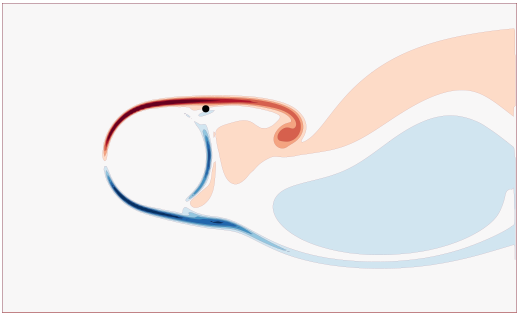
\includegraphics[width=\textwidth]{tex//fig/full_vort.png}
%     \end{subfigure}%
%     \begin{subfigure}{.5\textwidth}
%         \centering
%         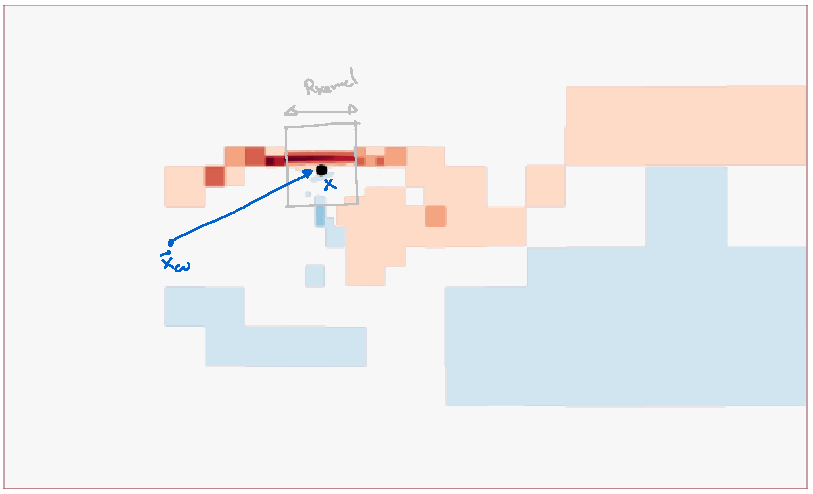
\includegraphics[width=\textwidth]{tex/fig/multilevel_vort.pdf}
%     \end{subfigure}
%     \caption{Vorticity field generated by the flow around a cylinder (left) and the Multilevel approach used to sample the vorticity field for a fast evaluation of the \emph{Biot-Savart} kernel at the black dot (right).}
%     \label{fig:ml_array}
% \end{figure}

We propose to replace the standard free-slip (or reflection) boundary conditions typically applied on the domain's exterior (Equ.~\ref{eq:BC_1} \& ~\ref{eq:BC_2}) by a \emph{Biot-Savart integral} of the vorticity inside the domain, implicitly assuming the flow external to the domain is irrotational (and that the flow is incompressible everywhere. This is the case for the flow around accelerated bodies, when the timescale follows $\frac{tU}{L}<\sim 4$. In this case, we can obtain the velocity induced by the vorticity contained within the domain at a point $\vec x$ on the boundary $\partial\Omega$ from a Green's function solution to the vorticity equation Eq.~\ref{eq:u_vort}
\begin{equation}\label{eq:Biot}
    {\vec u}({\vec x}) = f(\vec x; \vec\omega,\Omega) = \int_\Omega K_{n}({\vec x} - \vec{y})\times \vec\omega({\vec y})\text{ d}\vec{y} \quad\quad \forall \vec x\, \in \partial\Omega (N^{1/2})
\end{equation}
where $K_n$ is the $n$-dimensional Biot-Savart kernel. This kernel takes the following form \cite{Eldredge2019MathematicalFlows}
\begin{equation}
    2D:\quad K\equiv -\frac{\vec{r}}{2\pi|\vec{r}|^2}, \qquad\qquad 3D:\quad K\equiv -\frac{\vec{r}}{4\pi|\vec{r}|^3}.
\end{equation}

On a staggered grid, we need only apply the integral equation \ref{eq:Biot} to compute the velocity induced by the vorticity on the single component normal to the domain face. For ghost cells external to the computational domain, we use the local derivative conditions $\nabla\cdot\vec{u} = \nabla\times\vec{u}=0$ to compute the velocity. These conditions are consistent with the assumption that the flow is potential outside the domain, as well as being trivial to compute. Specifically, we apply the zero curl condition to all tangential velocity components in the ghost cells and then the zero divergence condition to the normal components in the ghost cells, marching away from the domain boundary.

% \begin{figure}
%     \centering
%     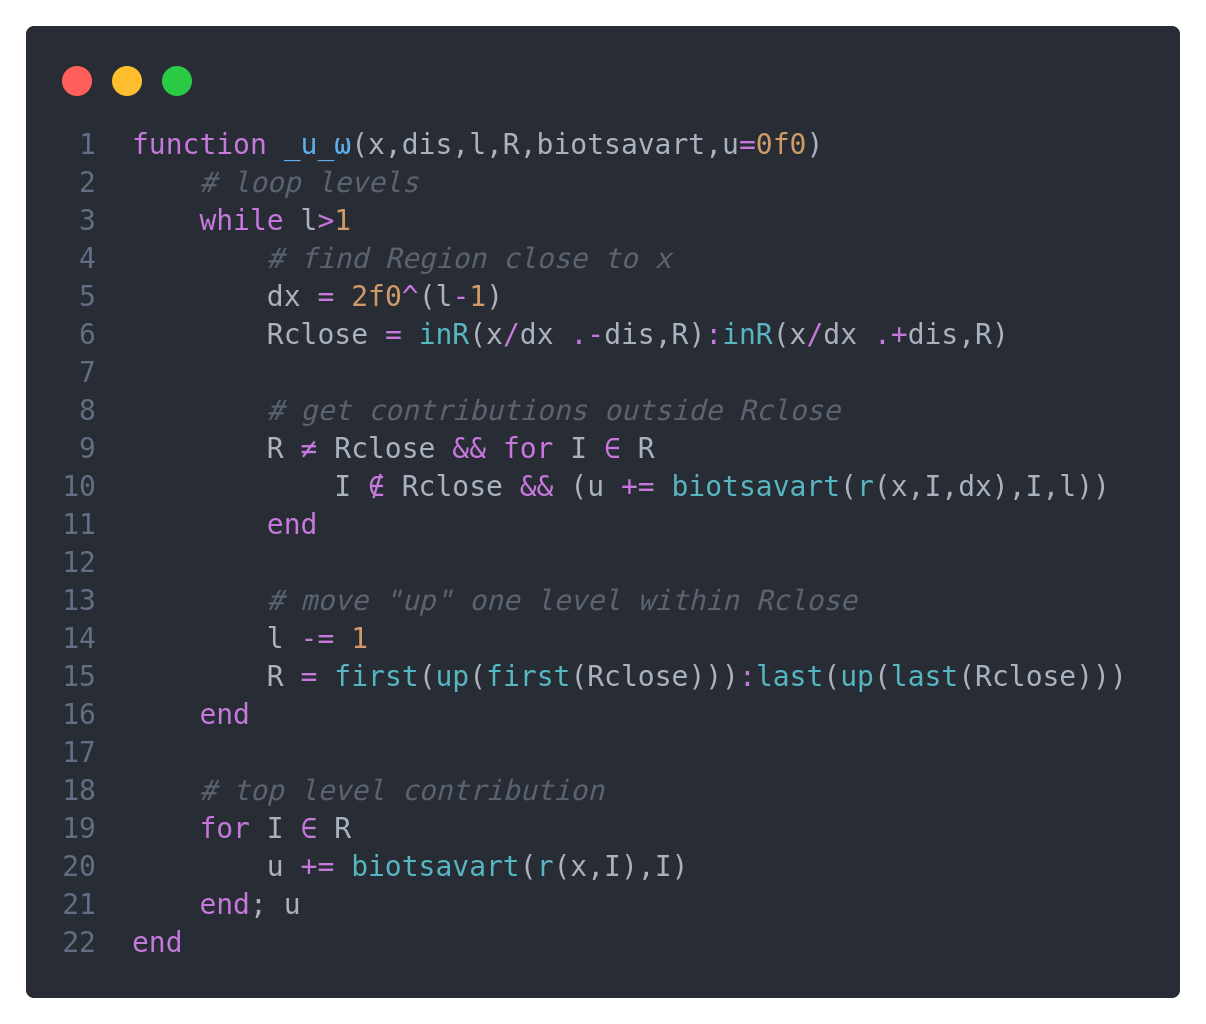
\includegraphics[width=0.5\linewidth]{tex//fig/code.png}
%     \label{fig:code_snippet}
%     \caption{Sample code}
% \end{figure}

\subsection{Fast evaluation of the Biot-Savart integral}

\begin{figure}
    \centering
    \def\svgwidth{0.8\columnwidth}
    \input{fig/multilevel_domain.pdf_tex}
    \caption{Schematic of the multilevel approach to evaluate the \emph{Biot-Savart} integral for a boundary point $\vec x$ over the nested domains $\mathcal{D}^{(1)} \cup \mathcal{D}^{(2)} \cup \mathcal{D}^{(3)} \cup \mathcal{D}^{(4)}$. The bounding box half-width on the finest level is shown as ${S}^{(1)}$. The computational domain $\Omega$ and its boundary $\partial\Omega$ and the immersed body $\mathcal{B}$ are shown. We also show a schematic of the coarsening of the grid between the domains. Domain and cell size are only for representation proposes.}
    \label{Fig_2}
\end{figure}

A key ingredient in our multilevel algorithm is the balance between accuracy and computational efficiency. The aim of this method is to reduce computational time compared to a large grid by providing a way of estimating the far-field boundary conditions. However, evaluation of these far-field boundary conditions has a significant cost. A naive evaluation of Eq.~\theequation~ would result in $N^{3/2}$ computation in two-dimensions and would be counter-productive in most cases. In vortex-particle methods, this infinite integral is standard and usually evaluated with \emph{Fast Multipole Method} that allows reducing this cost to $N^{1/2}\log N$ operations. Here, we use a multigrid algorithm to achieve the same reduction in operation.

% This is controlled by a criterion that triggers the evaluation of the velocity on progressively finer meshes. Given a point $x$ where the velocity induced by the vorticity blob located at $x_\omega$, the induced velocity is evaluated on the multilevel if the point $x_\omega$ falls in a box of size $\pm R_\text{kernel}$ around that point, see Fig.~\ref{fig:code_snippet}

We construct the multilevel Biot-Savart operator on the complete domain $\Omega$ by a $l$-level combination of gradually coarser meshes for each point $\vec x$ on the domain boundary $\partial \Omega$ (to avoid confusion between power and superscript index, we represent that later in parenthesis)
\begin{equation}\label{eq:multilevel}
    \Omega = \mathcal{D}^{(1)}(\vec x) \cup \mathcal{D}^{(2)}(\vec x) \cup \cdots \cup \mathcal{D}^{(l-1)}(\vec x) \cup \mathcal{D}^{(l)}(\vec x),
\end{equation}
where level $1$ is the finest domain and $l$ is the coarsest, and each domain is non-overlapping and their union fully covers $\Omega$, Fig \ref{Fig_2}. This decomposition is "centered" around the point of evaluation $\vec x$, meaning that the finest grid level is adjacent to $\vec x$ and the grid progressively coarsens as we move away. Therefore the contributions to equation \ref{eq:Biot} are more accurately calculated when close to $\vec x$, and the smaller contributions further from $\vec x$ are quickly estimated on the coarser levels.

In constructing these different domains, it is desirable that some moments of vorticity are conserved (to machine roundoff) \cite{Colonius2008}. Our multilevel implementation conserves the total circulation in the domain by a conservative interpolation of the vorticity from the finest level to the coarsest level
Following \ref{eq:multilevel}, the vorticity field in the domain can be expressed as a combination of gradually coarser vorticity fields
% \begin{equation}
%     \phi = \phi^{(1)} \cup \phi^{(2)} \cup \cdots \cup \phi^{(l-1)} \cup \phi^{(l)}
% \end{equation}
\begin{equation}
    \omega = \omega^{(1)} \cup \omega^{(2)} \cup \cdots \cup \omega^{(l-1)} \cup \omega^{(l)}
\end{equation}
see Fig.~\ref{Fig_2}. Where we have omitted the explicit location $\vec x$ in the different vorticity fields to imply that each of them covers the entire domain $\Omega$. The vorticity on the finest mesh is interpolated onto the coarser mesh via the restrictions operator
\begin{equation}
    \begin{split}
        \vec{\omega}^{(1)} &= \vec{\omega} \quad \forall\ \vec{y}\ ^{(1)} \in \mathcal{D}^{(1)}\\
        \vec{\omega}^{(i)} &= \mathcal{P}^{(i-1)\to(i)}\vec{\omega}^{(i-1)} \quad \forall\  \vec{y}\ ^{(i)} \in \mathcal{D}^{(i)}\\
    \end{split}
\end{equation}
where the restriction operator is uniform pooling from the $i-1$ level, see \cite{Weymouth2022Data-drivenProjection}.

With this finite $l$ set of non-overlapping domains $\mathcal{D}^{(i)}$ the integral in Eq.~\ref{eq:Biot} can be replaced with a sum over all the contribution from the domains at a point $\vec x$
\begin{equation}\label{eq:biot_sum}
    f(\vec{x}; \vec{\omega},\Omega) = \sum_{i=1}^{l} f(\vec{x}; \omega^{(i)},\mathcal{D}^{(i)}).
\end{equation}
To determine if the vorticity at a point $\vec y$ is evaluated on the $l^{th}$ level or a coarser level, we determine if point $\vec y$ lies within a bounding box, centered on $\vec x$ with half-width $S^{(l)}$. A point that lies within the box if all of its coordinates fall below that of $S^{(l)}$, that is $\text{all}(\vec{y}<{S}^{(l)})$. To avoid having to define a new bounding box dimension for each multilevel, we normalize ${S}^{(l)}$ with the cell size on that level $\Delta h^{(l)} = \Delta x^{(l)} = \Delta y^{(l)} (= \Delta z^{(l)}) = 2^{l-1}$ (two to the power of $l-1$), giving us a non-dimensional bounding box of half-width 
\begin{equation}\label{eq:bbox}
    \tilde{S} = \frac{{S}^{(l)}}{2^{1-l}},
\end{equation}
in what follows, we will assume that all dimensions compared to the bounding box are also normalized by cell size at that level.

The cost and accuracy of the summation in Eq.~\ref{eq:biot_sum} is linked to the dimensions of $\tilde{S}$

\paragraph{Analysis of error associated with a certain kernel}

We now discuss the choice of bonding box size $|\vec{S}|$ that maximizes the accuracy of the integral while reducing computational costs. From Fig~\ref{Fig_2}, it is clear that evaluation of the vorticity field onto the coarsest level will introduce smearing of any strong shear layer or vorticity blob. We show that with careful selection of $\vec{S}$, we can minimize these errors.

We start by assuming that the vorticity field on the finest level si exact. The choice of $\vec{S}$ will thus influence the error we make by approximating the induced velocity at a point $\vec y$ by evaluating it on gradually coarser meshes, compared to evaluating it on the finest mesh.

Within our multilevel algorithm, cells sufficiently far away is grouped with their neighbors to form a cell 4 times bigger in 2D and 8 times bigger in 3D. For simplicity, we discuss the 2D case, extensions to the 3D case are trivially obtained by alternating the out of plane vector, see below. Assuming the vorticity in these cells can be represented by point vortices with circulation $\Gamma_i$, the new (merged) point vortex now has circulation $\Gamma$ 
\begin{equation}
    \Gamma = \sum_{i=1}^{4}\Gamma_i,
\end{equation}
and is located at point $\vec{y}$. The induced velocity by this point vortex at location $\vec x$, is thus given by
\begin{equation}\label{eq:induced_1}
    \vec{u}(\vec{x}) = \frac{\vec{y}-\vec{x}}{2\pi|\vec{y}-\vec{x}|^2}\times\vec{e}_z\Gamma = \frac{\vec{r}}{2\pi|\vec{r}|^2}\times\vec{e}_z\sum_{i=1}^{4}\Gamma_i
\end{equation}
where we have substituted $\vec{r}=\vec{y}-\vec{x}$ and $\vec{e}_z$ the the out-of-plane unit vector. For 3D flow, each component can be reconstructed by alternating the out-of-plane vector between $\vec{e}_x$, $\vec{e}_y$ and $\vec{e}_z$ and using the corresponding vorticity component. The actual velocity induced by these four point-vortices (before we grouped them) is given by
\begin{equation}
    \vec{u}^e(\vec{x}) = \sum_{i=1}^{4}\frac{\vec{r}_i}{2\pi|\vec{r}_i|^2}\times\vec{e}_z\Gamma_i,
\end{equation}
where $\vec{r}_i=\vec{y}_i-\vec{x}$. We can further decompose this expression by noting that $\vec{r}_i=\vec{y}-\vec{x}-\vec{\delta r}_i=\vec{r}-\vec{\delta r}_i$, where $\vec{y}$ is the position of the geometric center of the 4 point vortex (where we merge them into the bigger one). Substitution in Eq.~\theequation~ gives
\begin{equation}
    \vec{u}^e(\vec{x}) = \sum_{i=1}^{4}\frac{\vec{r}-\vec{\delta r}_i}{2\pi|\vec{r}-\vec{\delta r}_i|^2}\times\vec{e}_z\Gamma_i.
\end{equation}
For sufficiently large $\vec{r}$ we can assume that $|\vec{r}|\approx|\vec{r}-\vec{\delta r}_i|$ %and thus we have
% \begin{equation}
%     \vec{u}^e(\vec{x}) = \sum_{i=1}^{4}\frac{\vec{r}-\vec{\delta r}_i}{2\pi|\vec{r}|^2}\times\vec{e}_z\Gamma_i.
% \end{equation}
which allows us to separate the kernel's influence into two parts
\begin{equation}
    \vec{u}^e(\vec{x}) = \sum_{i=1}^{4}\frac{\vec{r}}{2\pi|\vec{r}|^2}\times\vec{e}_z\Gamma_i-\sum_{i=1}^{4}\frac{\vec{\delta r}_i}{2\pi|\vec{r}|^2}\times\vec{e}_z\Gamma_i.
\end{equation}
After rearrangement, the first term equals Equ.~\ref{eq:induced_1}. The second term is the error we make by approximating the integral over numerous points by one over a single point-vortex. In the limit of extremely fine grid ($|\delta \vec{r}_i|=0$) or zero vorticity ($\Gamma_i=0$) away from the point of evaluation, this error vanishes, as expected. 

Ultimately, we are interested in the magnitude of this error
\begin{equation}
    \varepsilon(\vec{x}) = \sum_{i=1}^{4}\vert\frac{\vec{\delta r}_i}{2\pi|\vec{r}|^2}\times\vec{e}_z\Gamma_i\vert = 
    \sum_{i=1}^{4}\frac{\vert\vec{\delta r}_i\vert}{2\pi|\vec{r}|^2}\Gamma_i,
\end{equation}
as $\vec{e}_z$ does not contribute to the magnitude of the error. On uniform Cartesian meshes, we can relate the distance from the $i^{th}$ point-vortex to the cell center with the grid size on the $l$-level, $\vert\vec{\delta r}_i^{(l)}\vert=2^{l-3/2}$ (similarly in 3D we get $\vert\vec{\delta r}_i^{(l)}\vert=2^{l-3/2}\sqrt{3}$). The error introduced by the multilevel pooling of the vorticity field on the $l$-level is
\begin{equation}
    \varepsilon(\vec{x})^{(l)} = \sum_{i=1}^{4(l-1)}\frac{2^{l-3/2}}{2\pi|\vec{r}|^2}\Gamma_i.
\end{equation}
% \begin{equation}
%     \varepsilon(\vec{x})^{(l)} = \sum_{i=1}^{4(l-1)}\frac{\sqrt{2}\Delta x}{4\pi|\vec{r}|^2}\Gamma_i=\frac{\sqrt{2}\Delta x}{4\pi|\vec{r}|^2}\sum_{i=1}^{4}\Gamma_i,
% \end{equation}
The level at which the vorticity is evaluated depends on the bounding box $\tilde{S}$ at each level. This criterion provides an upper bound for the error carried from level $l$ onto the induced velocity at $\vec x$ as $|\vec{r}|^2 \approx 2^{2l-2}\tilde{S}^2$ using Equ.~\ref{eq:bbox}. The upper bound error is
\begin{equation}
    \varepsilon(\vec{x})^{(l)} = \frac{2^{l-3/2}}{2\pi\cdot2^{2l-2}\cdot\tilde{S}^2}\sum_{i=1}^{4(l-1)}\Gamma_i = \frac{2^{3/2}}{2^{l}\pi\tilde{S}^2}\sum_{i=1}^{4(l-1)}\Gamma_i.
\end{equation}
Finally, the upper bound for the total error in the induced velocity at a point $\vec x$ due to the $l$-level evaluation of the \emph{Biot-Savart} integral is
\begin{equation}
    \varepsilon(\vec{x}) = \sum_{l=1}^{N_l}\frac{2^{3/2}}{2^{l}\pi\tilde{S}^2}\sum_{i=1}^{4(l-1)}\Gamma_i = \frac{2^{3/2}}{\pi\tilde{S}^2}\sum_{l=1}^{N_l}\frac{1}{2^l}\sum_{i=1}^{4(l-1)}\Gamma_i.
\end{equation}
which decays as $\tilde{S}^{-2}$. As expected, taking $\tilde{S}>\text{Domain}$ yields $\varepsilon(\vec{x}) = 0$, and as $\Gamma_i \to 0, \varepsilon(\vec{x})\to 0$, finally as $\tilde{S}\to0, \varepsilon(\vec{x}) \to \infty$. Similarly, in 3D the error is given by
\begin{equation}
    \varepsilon(\vec{x}) = \frac{2^{3/2}\sqrt{3}}{\pi\tilde{S}^3}\sum_{l=1}^{N_l}\frac{1}{2^{l}}\sum_{i=1}^{8(l-1)}\Gamma_i.
\end{equation}
which decays as $\tilde{S}^{-3}$. 

The cost of the evaluation of the \emph{Biot-Savart} integral is also proportional to the bounding box dimension. Each level contains approximately $\tilde{S}^d$ points, with $d$ the dimension of the problem. Using a $l$-level mutligrid will result in roughly $\tilde{S}^d\times l$ operations. The maximum number of levels is given by $l=N/\tilde{S}$. The total cost is thus $\tilde{S}^{d-1}N$

which is much lower than the total number of operations required to evaluate Equ.~\ref{eq:Biot} without a multilevel approach.


% Let $\vec{S}^{l}$ be the distance criterion on level $l$, the total error is a sum of all the errors in the $N_l$ lower level of the multigrid
% \begin{equation}
%     \varepsilon^{(1)}(\vec{x}) = \sum_{l=2}^{N_l}\frac{\sqrt{2}\Delta x^{(l-1)}}{4\pi|\vec{S}^{(l-1)}|^2}\sum_{i=1}^{4l}\Gamma_i.
% \end{equation}

% As expected, taking $\vec{S}>\text{Domain}$ yiels $\varepsilon^{(1)}(\vec{x}) = 0$, and as $\Gamma_i \to 0, \varepsilon^{(1)}(\vec{x})\to 0$, finally as $|\vec{S}|\to0, \varepsilon^{(1)}(\vec{x}) \to \infty$. Similarly, in 3D the error is given by
% \begin{equation}
%     \varepsilon^{(1)}(\vec{x}) = \sum_{l=2}^{N_l}\frac{\sqrt{3}\Delta x^{(l-1)}}{16\pi|\vec{S}^{(l-1)}|^3}\sum_{i=1}^{8l}\Gamma_i,
% \end{equation}
% which decays much faster than in 2D.

Lastly, we note that this multilevel error implies that global mass conservation is no longer guaranteed on the domain boundary. As such, we apply a uniform correction which will be proportional to the average error discussed above
\begin{equation}
    \vec{u} = \vec{u} -\frac {\oint_{\partial\Omega }\hat{n}\cdot\vec{u}\text{ d}S} {\oint_{\partial\Omega }\text{ d}S}.
\end{equation}
ensuring a globally divergence-free boundary conditions.


% The integral in Eq.~\ref{eq:Biot} is then evaluated by the recursive expression, starting from the lowest level of the multigrid
% \begin{equation}
%     f^{(l)}(\vec{x},\vec{y},\vec{\omega}^{(l)}) = \begin{cases}
%         \sum_{\vec{y}\in\mathcal{D}^{(l)}}K^{(l)}(\vec{x},\vec{y},\vec{\omega}^{(l)}), \quad \forall \,\, \vec{y} \in \mathcal{D}^{(l)}\\
%         f^{(l-1)}(\vec{x},\vec{y},\vec{\omega}^{(l-1)}), \,\,\qquad \text{else},
%     \end{cases}
% \end{equation}
% where $K^{(l)}(\vec{x},\vec{y},\vec{\omega}^{(l)})$ is the discrete \emph{Biot-Savart} kernel at level $l$ and the criterion $\vec{y} \in \mathcal{D}^{(l)}$ is evaluated using a standard cut-of radius.
% \begin{equation}
%     \begin{cases}|\vec{y}-\vec{x}|/2^l<|\vec{S}|, \qquad \vec{y} \in \mathcal{D}^{(l)},\\
%     |\vec{y}-\vec{x}|/2^l>|\vec{S}|, \qquad \vec{y} \notin \mathcal{D}^{(l)}.
%     \end{cases} 
% \end{equation}

% \textbf{Must be a bounding box and not a cut-off radius}
% \textbf{Still need to show the cost to evaluate integral is logN. $S^2*l$}

\subsection{Biot-Savart \& Projection Algorithm}\label{sec:Biot_projection}
Substitution of the \emph{Biot-Savart} boundary condition (Eq.~\ref{eq:Biot}) into the projection scheme results in a slightly modified intermediate velocity field\\
\textbf{Biot-Savart intermediate step}
\begin{align}
    &\vec{u}^* = \vec{u}\,^t + \int_{t}^{t+\Delta t}\frac{1}{Re}\nabla^2\vec{u} -\left(\vec{u}\cdot\nabla\right)\vec{u}\text{ d}t &\quad\forall\ \vec{x}\in\Omega (N),\\
    &\vec{u}^* = f(\vec{x},\nabla\times \vec{u}^*,\Omega) &\quad\forall\ \vec{x}\in\partial\Omega (N^{1/2})
\end{align}
where the exterior boundary condition have been computed from the intermediate velocity $\vec{u}^*$ in the domain. The projection step, however, results in a coupling between the body and the domain's boundary through the pressure field
\begin{align}
  &\nabla\cdot\frac{\Delta t}{\rho}\nabla p = \nabla\cdot \vec{u}^* &\forall\ \vec{x}\in\Omega (N)\\
  &\vec{u}^{t+\Delta t} = \vec{u}^*-\frac{\Delta t}{\rho}\nabla p &\quad\forall\ \vec{x}\in\Omega (N)\\
  &\vec{u}^{t+\Delta t} = f(\vec{x},\nabla\times \vec{u}^{t+\Delta t},\Omega)= \vec{u}^*-f(\vec{x},\nabla\times\frac{\Delta t}{\rho}\nabla p,\Omega) &\quad\forall\ \vec{x}\in\partial\Omega (N^{1/2}).
\end{align}
Away from the body, the source term in the \emph{Biot-Savart} integral in Equ.~\theequation~ vanishes> However, due to the pressure boundary condition on the immersed body ($\partial p/\partial\hat{n}=\text{d}\vec{U}_b/\text{d}t$), a thin layer of vorticity is generated by the pressure gradient term that changes the induced velocity field on the outer domain's boundary. The projection steps and the \emph{Biot-Savart} boundary conditions now form a fixed-point system

\textbf{Biot-Savart projection step}
\begin{align}
    &\nabla\cdot\frac{\Delta t}{\rho}\nabla p = \nabla\cdot \vec{u}^*-\nabla\cdot f(\vec{x},\nabla\times\frac{\Delta t}{\rho}\nabla p,\Omega) &\quad\forall\ \vec{x}\in\Omega, \vec{x}\in\partial\Omega\ (N)\\
    &\vec{u}^{t+\Delta t} = \vec{u}^*-\frac{\Delta t}{\rho}\nabla p &\quad\forall\ \vec{x}\in\Omega (N)\\
    &\vec{u}^{t+\Delta t} = f(\vec{x},\nabla\times \vec{u}^{t+\Delta t},\Omega)= \vec{u}^*-f(\vec{x},\nabla\times\frac{\Delta t}{\rho}\nabla p,\Omega) &\quad\forall\ \vec{x}\in\partial\Omega (N^{1/2}).
\end{align}
This coupling only occurs on the domain's boundary, and the resulting system is mildly non-linear. This weak non-linearity can be solved efficiently with the deferred correction method and does not require Newton-type methods that will prevent us from using a standard Poisson solver for the pressure. An explicit update of the source term of the Poisson problem during each pressure solver iteration ensures that the divergence-free constraint is respected and that this thin layer of vorticity is properly accounted for. In immersed boundary methods, this coupling is only apparent if the pressure boundary conditions are correctly imposed on the immersed body during the projection step; see for example \cite{Taira2007, Lauber2022}.

\section{Multilevel reconstruction validation}

We start by validating the multilevel reconstruction algorithm presented above. We selected to cases such respect our assumption of vorticity being confined far from the domain's boundary. We demonstrate the 2D and 3D reconstruction error of the multilevel and the speedup generated by selecting the correct kernel radius from the above analysis.

Our \emph{Biot-Savart} boundary conditions are implemented inside \textbf{\color{cyan}{{WaterLily.jl}}}\footnote{\url{https://github.com/weymouth/WaterLily.jl}}, a fast, immersed-boundary flow solver based on the Boundary data immersion method \cite{Maertens2015} that can execute both on CPU and GPU \cite{Weymouth2023WaterLily.jl:Execution}. To leverage the GPU capability of the flow solver and fully benefit from our novel boundary conditions, we perform all computations presented herein on an NVIDIA-A6000 GPU (48GB memory). All the codes used for this study and the instructions to reproduce these results are freely available at \url{https://github.com/weymouth/BiotSavartBCs.jl}.

\subsection{2D validation: Lamb vortex}

The velocity field generated by the Lamb-Chaplygin dipole is obtained from the scalar stream function $\vec{u} = -\vec{e}_z\times \nabla \psi$ given by
\begin{equation}
    \psi(r) = \begin{cases}
    \frac{-2UJ_1(\beta r)}{\beta J_0(\beta R)}, \quad \text{for} \quad r < R,\\
    U\left(\frac{R^2}{r}-r\right), \quad \text{for} \quad r \ge R,    \end{cases}
\end{equation}
%Meleshko, V. V.; Heijst, G. J. F. van (August 1994). "On Chaplygin's investigations of two-dimensional vortex structures in an inviscid fluid". Journal of Fluid Mechanics. 272: 157–182. Bibcode:1994JFM...272..157M. doi:10.1017/S0022112094004428. ISSN 1469-7645. S2CID 123008925.
where $J_0$ and $J_1$ are the zeroth and first Bessel functions of the first kind, respectively. $\beta$ is a parameter with the value $\beta=1.2197\pi/R$. The vortex posses an \emph{atmosphere}, defined by the isoline $\psi(r=R)=0$, that delimits the inside and outside of the vortex.


\begin{figure}
\begin{subfigure}{.5\textwidth}
  \centering
  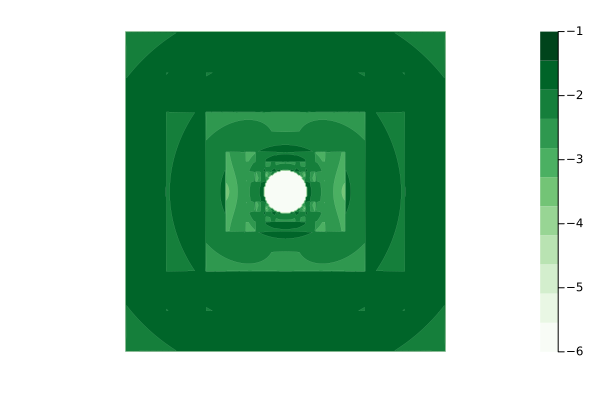
\includegraphics[width=\linewidth]{tex/fig/lamb_dipole_error_dist2.png}
  \caption{}
\end{subfigure}%
\begin{subfigure}{.5\textwidth}
  \centering
  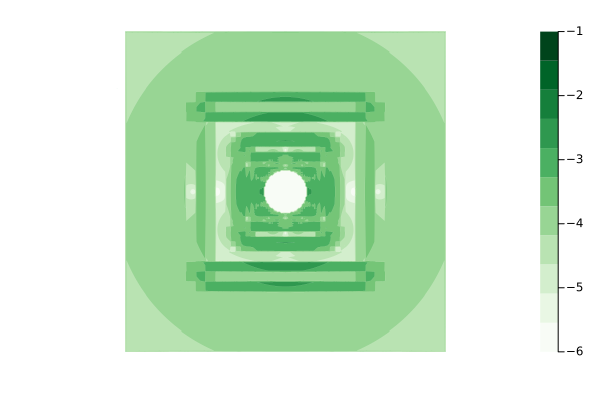
\includegraphics[width=\linewidth]{tex/fig/lamb_dipole_error_dist8.png}
  \caption{}
\end{subfigure}
\begin{subfigure}{.5\textwidth}
  \centering
  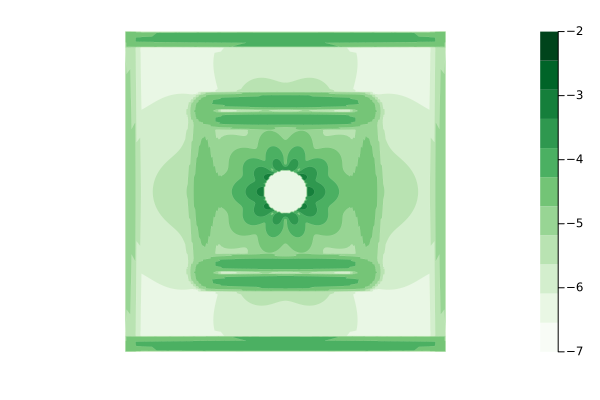
\includegraphics[width=\linewidth]{tex/fig/lamb_dipole_error_dist32.png}
  \caption{}
\end{subfigure}%
\begin{subfigure}{.5\textwidth}
  \centering
  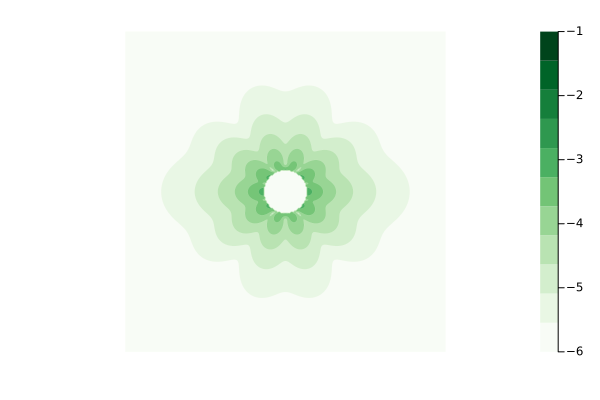
\includegraphics[width=\linewidth]{tex/fig/lamb_dipole_error_dist128.png}
  \caption{}
\end{subfigure}
\caption{$L_2$-norm of the error in reconstructed velocity field outside the atmosphere of the 2D Lamb-Chaplygin vortex for varying (multi-level) kernel size. Error bars are shown in log-scale.}
\label{fig:lam_error_dist}
\end{figure}

We reconstruct the velocity field outside the vortex's atmosphere using the internal vorticity and our multilevel Biot-Savart method and compare that to the analytic result. The dependency of the absolute error in the reconstructed velocity field on the radius of the multilevel refinement criterion are shown in Fig.~\ref{fig:lam_error_dist}. Setting the refine size $\tilde{S}$ to the domain size $\cal D$ eliminates the multi-level-error, but the result is not exact since the analytic vorticity distribution is sampled on a finite grid of size $\Delta x=0.05
R$. This error depends primarily on the distance from the vortex, Fig.~\ref{fig:lam_error_dist}(d). Progressively reducing the refinement size $S/\Delta x$ introduces the multilevel error quantified in the previous section, which is only weakly dependant on the distance to the vortex.

This is further quantified in Fig.~\ref{fig:error_lamb_2}(a) which shows the maximum error in the reconstructed velocity field at distance $d$ from the vortex from the Lamb-Chaplygin vortex. The size $S/\Delta x$ is show to dominate the reconstruction error, with a fairly uniform total error levels once $S/\Delta x \le 2^3 = 8$. Fig.~\ref{fig:error_lamb_2}(a) reports the measure computational speed-up acheived by the multilevel method relative to setting $S=\cal D$, demonstrating up to 300x acceleration.

\begin{figure}
    \centering
    \begin{subfigure}{.5\textwidth}
        \centering
        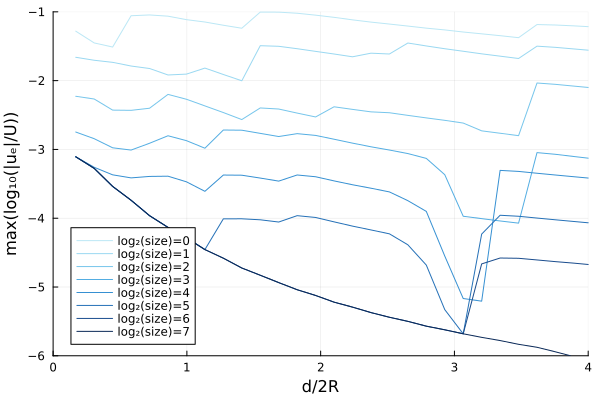
\includegraphics[width=\textwidth]{tex//fig/lamb_dipole_error_dists.png}
    \end{subfigure}%
    \begin{subfigure}{.5\textwidth}
        \centering
        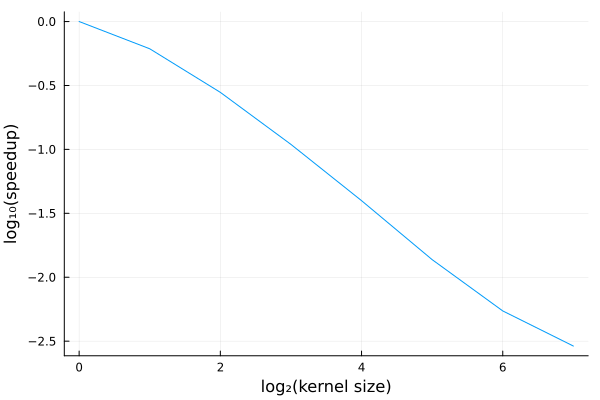
\includegraphics[width=\textwidth]{tex/fig/lamb_dipole_speedup_dists.png}
    \end{subfigure}
    \caption{Maximum error in the reconstructed velocity field generated by a 2D \emph{Lamb-Chaplygin} vortex dipole for various kernel sizes ($\tilde{S}$) and distances from the vortex core (left). Corresponding speed-up obtained by reducing the kernel size for the multigrid algorithm (right).}
    \label{fig:error_lamb_2}
\end{figure}

\subsection{3D validation: Hill vortex}

This validation is repeated in 3D using the classical \emph{Hill vortex}, whose radial and tangential velocity components are given by
\begin{align}
    v_r &= \frac{1}{r^2\sin\theta}\frac{\partial\psi}{\partial\theta}, \qquad v_\theta = -\frac{1}{r\sin\theta}\frac{\partial\psi}{\partial r}.
\end{align}
and the stream function 
\begin{equation}
    \psi(r,\theta) = \begin{cases}
    -\frac{3U}{4}\left(1-\frac{r^2}{R^2}\right)r^2sin^2\theta \quad \text{for} \, r \le R,\\
     \,\,\frac{U}{2}\left(1-\frac{r^3}{R^3}\right)r^2sin^2\theta \quad \text{for} \, r > R.
    \end{cases}
\end{equation}
with the corresponding errors and speed up shown in Figure~\ref{fig:error_hill_3}. Note that the analytic vorticity of the hill vortex is discontinuous, increasing the truncation error near the vortex compared to the smooth Lamp-vortex, a problem which would not be observed with any real three-dimensional viscous flow.

As argued in Sec.~\ref{sec:Biot_projection} the multilevel error decreases extremely quickly as $S/\Delta x$ is increased for three-dimensional flows. This is due to the scaling of the \emph{Biot-Savart} kernel itself. Similarly, the speed-up is much faster in 3D because each doubling gathers 8 cells instead of 4, with a max observed speed-up of nearly 20,000x using the multilevel method.

\begin{figure}
    \centering
    \begin{subfigure}{.5\textwidth}
        \centering
        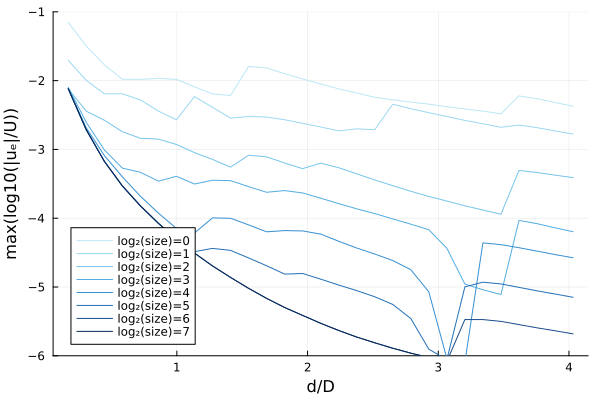
\includegraphics[width=\textwidth]{tex//fig/Hill_error_dists.png}
    \end{subfigure}%
    \begin{subfigure}{.5\textwidth}
        \centering
        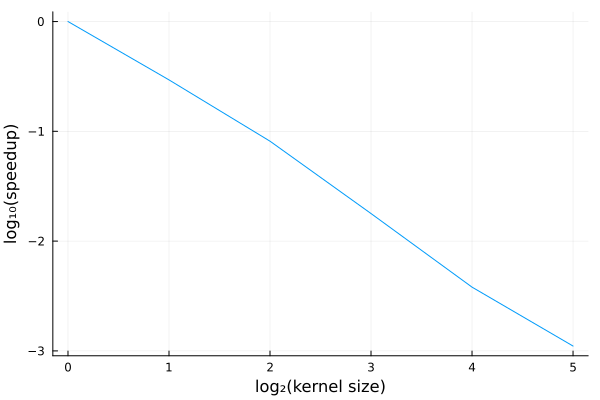
\includegraphics[width=\textwidth]{tex/fig/Hill_speedup_dists.png}
    \end{subfigure}
    \caption{Maximum error in the reconstructed velocity field generated by a 3D \emph{Hill} vortex for various kernel sizes ($\tilde{S}$) and distances from the vortex core (left). Corresponding speed-up obtained by reducing the kernel size for the multigrid algorithm (right).}
    \label{fig:error_hill_3}
\end{figure}

\section{Confined vorticity applications}

We next validate the application of the Bio-Savart conditions to the solution of a set of impulsive flow problems. The flow is truly irrotational outside the computational domain, matching the implicit assumptions required to use the Biot-Savart equations to reconstruct the velocity on the boundary. 

\subsection{3D flow around an accelerating disk}

The flow around a disk accelerated from rest in a quiescent flow is purely potential for $t\to 0^+$. As a result, an analytical expression for the added mass coefficient and the pressure field can be used to validate our novel potential flow boundary condition when injected in a moment step of the \emph{Navier-Stokes} equations. We place a disk of radius $R$ in an initially quiescent flow. The disk is prescribed with a constant acceleration $a$ during one non-dimensional time $t^*=at/U$
\begin{equation}
    U(t) = \begin{cases}
        at, \quad \text{if } at/U\le1,\\
        U, \quad \text{else}.
    \end{cases}
\end{equation}
We integrate the Navier-Stokes equation during a single time-step from $t=0\to0^+$ and compute the pressure force acting on the disk for various domain sizes. From potential flow theory, the added-mass coefficient for an impulsively started flow is
\begin{equation}
    Ca  = \frac{F_{am}}{\rho D^3 a} = \frac{F_{am}}{\rho D^2U^2}\left(\frac{1}{a^*}\right) = \frac{1}{3}
\end{equation}
where $Ca$ is the classical added-mass coefficient for a circular plate. We then continue the simulation until $t^*=3$. Once the disk reaches its peak velocity, the Reynolds number is $Re=\frac{UR}{\nu}=1000$. 

Figure~\ref{fig:disk_flow_1}-\ref{fig:disk_flow_2} shows the vorticity and pressure field at three consecutive times during the cylinder's motion. Fig.~\ref{fig:disk_flow_1} show the results with the standard reflective boundary conditions (the entire computational domain is shown), and in Fig.~\ref{fig:disk_flow_2}, the flow has been obtained with the \emph{Biot-Savart} boundary conditions. High blockage effects are apparent for the reflective boundary conditions, with stronger shear layers and a vortex center located further downstream than the \emph{Biot-Savart} results. The pressure field is even more striking. With iso-contour of the pressure sticking to the wall to satisfy the homogeneous Neumann condition set by the velocity field, see \cite{}. Because the \emph{Biot-Savart} boundary conditions improve this boundary condition, the pressure follows the expected potential flow solution and, more importantly, is relaxed from the homogeneous Neumann condition that reflective boundary conditions imposed.

\begin{figure}
    \centering
    \begin{subfigure}{.33\textwidth}
        \centering
        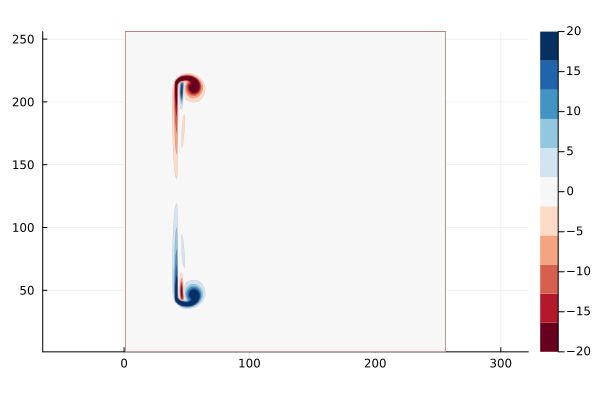
\includegraphics[trim={4cm 7.2cm 5cm 1cm},clip,width=\textwidth]{tex/fig/Disk_reflect_omega_1.png}
        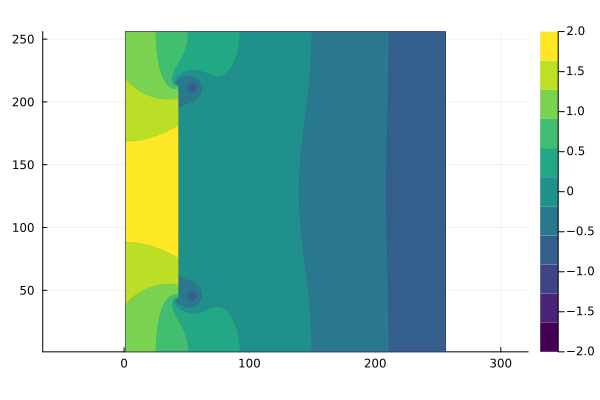
\includegraphics[trim={4cm 1.5cm 5cm 7cm},clip,width=\textwidth]{tex/fig/Disk_reflect_press_1.png}
    \end{subfigure}%
    \begin{subfigure}{.33\textwidth}
        \centering
        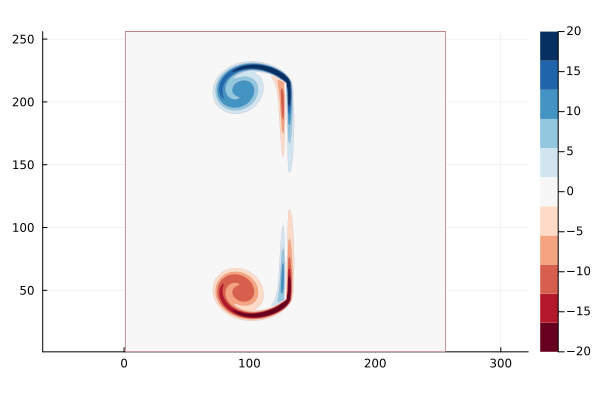
\includegraphics[trim={4cm 7.2cm 5cm 1cm},clip,width=\textwidth]{tex/fig/Disk_reflect_omega_2.png}
        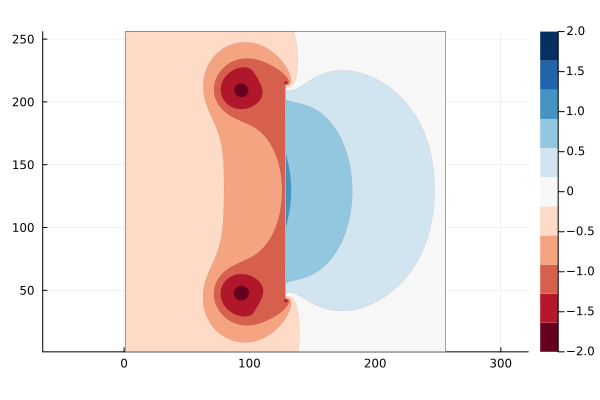
\includegraphics[trim={4cm 1.5cm 5cm 7cm},clip,width=\textwidth]{tex/fig/Disk_reflect_press_2.png}
    \end{subfigure}%
    \begin{subfigure}{.33\textwidth}
        \centering
         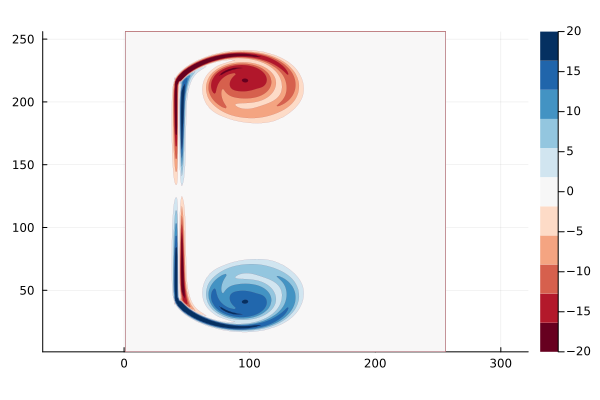
\includegraphics[trim={4cm 7.2cm 5cm 1cm},clip,width=\textwidth]{tex/fig/Disk_reflect_omega_3.png}
        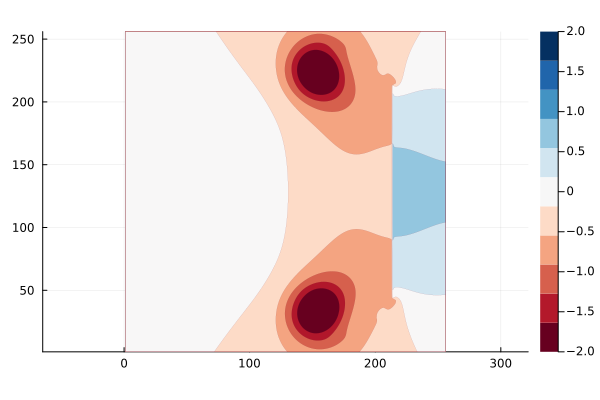
\includegraphics[trim={4cm 1.5cm 5cm 7cm},clip,width=\textwidth]{tex/fig/Disk_reflect_press_3.png}
    \end{subfigure}
    \caption{Flow around an initially stationary disk accelerated in a quiescent flow at three convective times, $t^*\in [1,2,3]$, using the reflective boundary conditions. The entire computational domain is shown. The top half shows 10 iso-contour of the vorticity, equally spaced in the interval $\omega L/U\in\pm20$. The bottom half shows the pressure field, with 10 iso-contour equally spaced in $p/\rho U^2\in\pm2$.}
    \label{fig:disk_flow_1}
\end{figure}

Zero point for time. Xu and Nietsche paper 2015.

Fig.~\ref{fig:disk_forces} shows the time trace of the pressure force acting on the accelerated disk. The difference in the pressure field is found again in the difference in the forces. Here, the \emph{Biot-Savart} boundary condition can exactly recover the added-mass force on the first time step, while the reflective boundary condition overestimates it. For larger $t^*$, the effect of the boundary condition is still observable; the reflective boundary condition significantly overestimates the pressure forces

\begin{figure}
    \centering
    \begin{subfigure}{.33\textwidth}
        \centering
         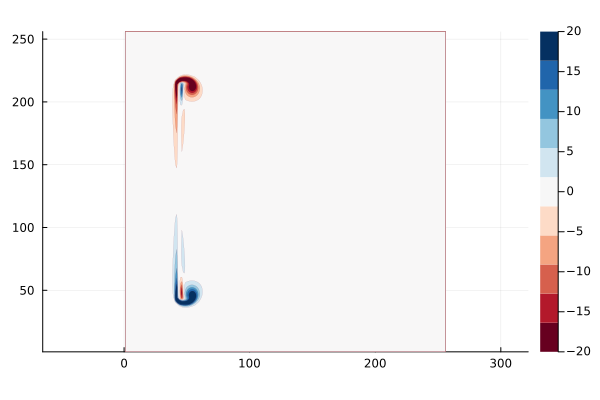
\includegraphics[trim={4cm 7.2cm 5cm 1cm},clip,width=\textwidth]{tex/fig/Disk_biot_omega_1.png}
        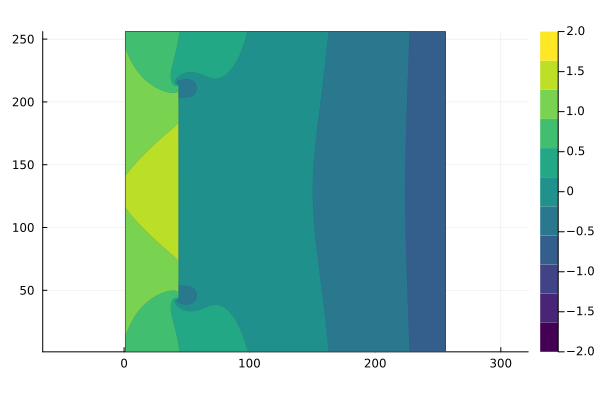
\includegraphics[trim={4cm 1.5cm 5cm 7cm},clip,width=\textwidth]{tex/fig/Disk_biot_press_1.png}
    \end{subfigure}%
    \begin{subfigure}{.33\textwidth}
        \centering
        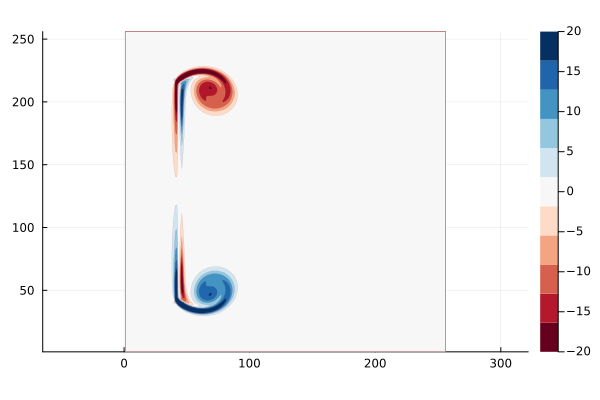
\includegraphics[trim={4cm 7.2cm 5cm 1cm},clip,width=\textwidth]{tex/fig/Disk_biot_omega_2.png}
        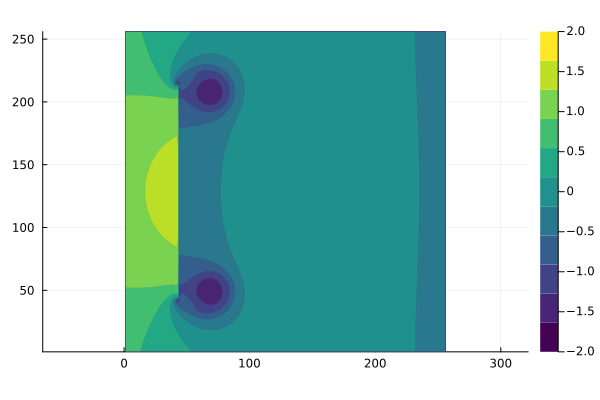
\includegraphics[trim={4cm 1.5cm 5cm 7cm},clip,width=\textwidth]{tex/fig/Disk_biot_press_2.png}
    \end{subfigure}%
    \begin{subfigure}{.33\textwidth}
        \centering
         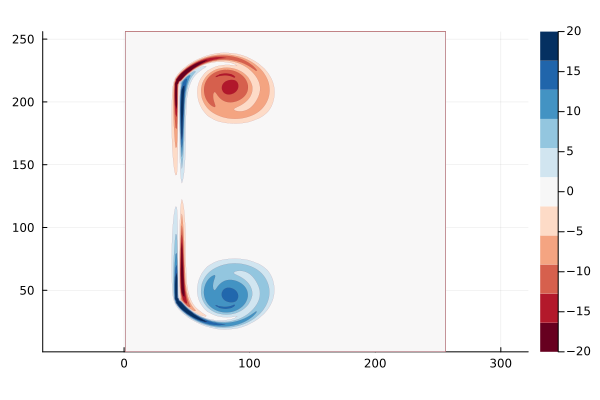
\includegraphics[trim={4cm 7.2cm 5cm 1cm},clip,width=\textwidth]{tex/fig/Disk_biot_omega_3.png}
        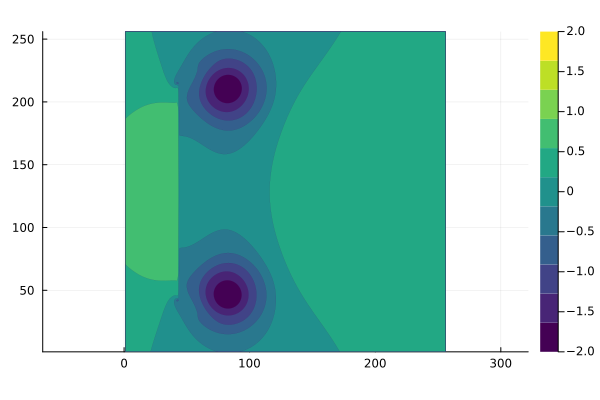
\includegraphics[trim={4cm 1.5cm 5cm 7cm},clip,width=\textwidth]{tex/fig/Disk_biot_press_3.png}
    \end{subfigure}
    \caption{Flow around an initially stationary disk accelerated in a quiescent flow at three convective times, $t^*\in [1,2,3]$, using the \emph{Biot-Savart} boundary conditions. The entire computational domain is shown. The top half shows 10 iso-contour of the vorticity, equally spaced in the interval $\omega L/U\in\pm20$. The bottom half shows the pressure field, with 10 iso-contour equally spaced in $p/\rho U^2\in\pm2$.}
    \label{fig:disk_flow_2}
\end{figure}


\begin{figure}
    \centering
    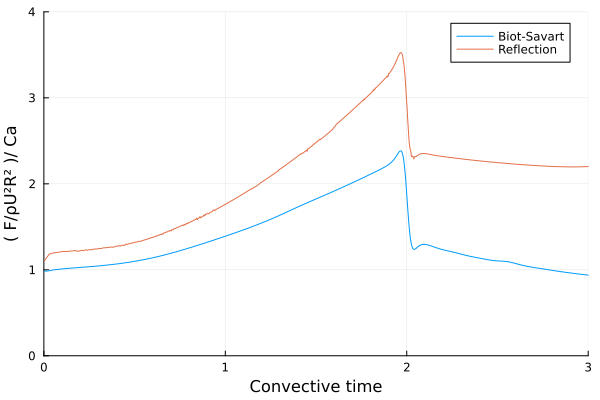
\includegraphics[width=0.5\textwidth]{tex//fig/Disk_256D_force.png}
    \caption{Instantaneous pressure force acting on the disk for the two different boundary conditions. The convective time corresponds to the snapshots shown in Fig.~\ref{fig:disk_flow_1}-\ref{fig:disk_flow_2}.}
    \label{fig:disk_forces}
\end{figure}


\subsection{3D Flow around a square disk at $Re=125\,000$}

To demonstrate the ability of our method to deal with highly separated and turbulent vortex formation, we simulate the flow around a square plate of dimension $L\times L$, accelerated in the surface normal direction to a final Reynolds number $Re=125\,000$. We focus on the initial vortex formation and position the plate at the center of a domain of size $2L\times2L\times2L$. For $t^*<6$, vortices typically stay attached to the body and only separate and travel downstream later, allowing us to use our \emph{Biot-Savart} boundary conditions for this build-up phase. 

\begin{figure}
    \centering
    \begin{subfigure}{.33\textwidth}
        \centering
        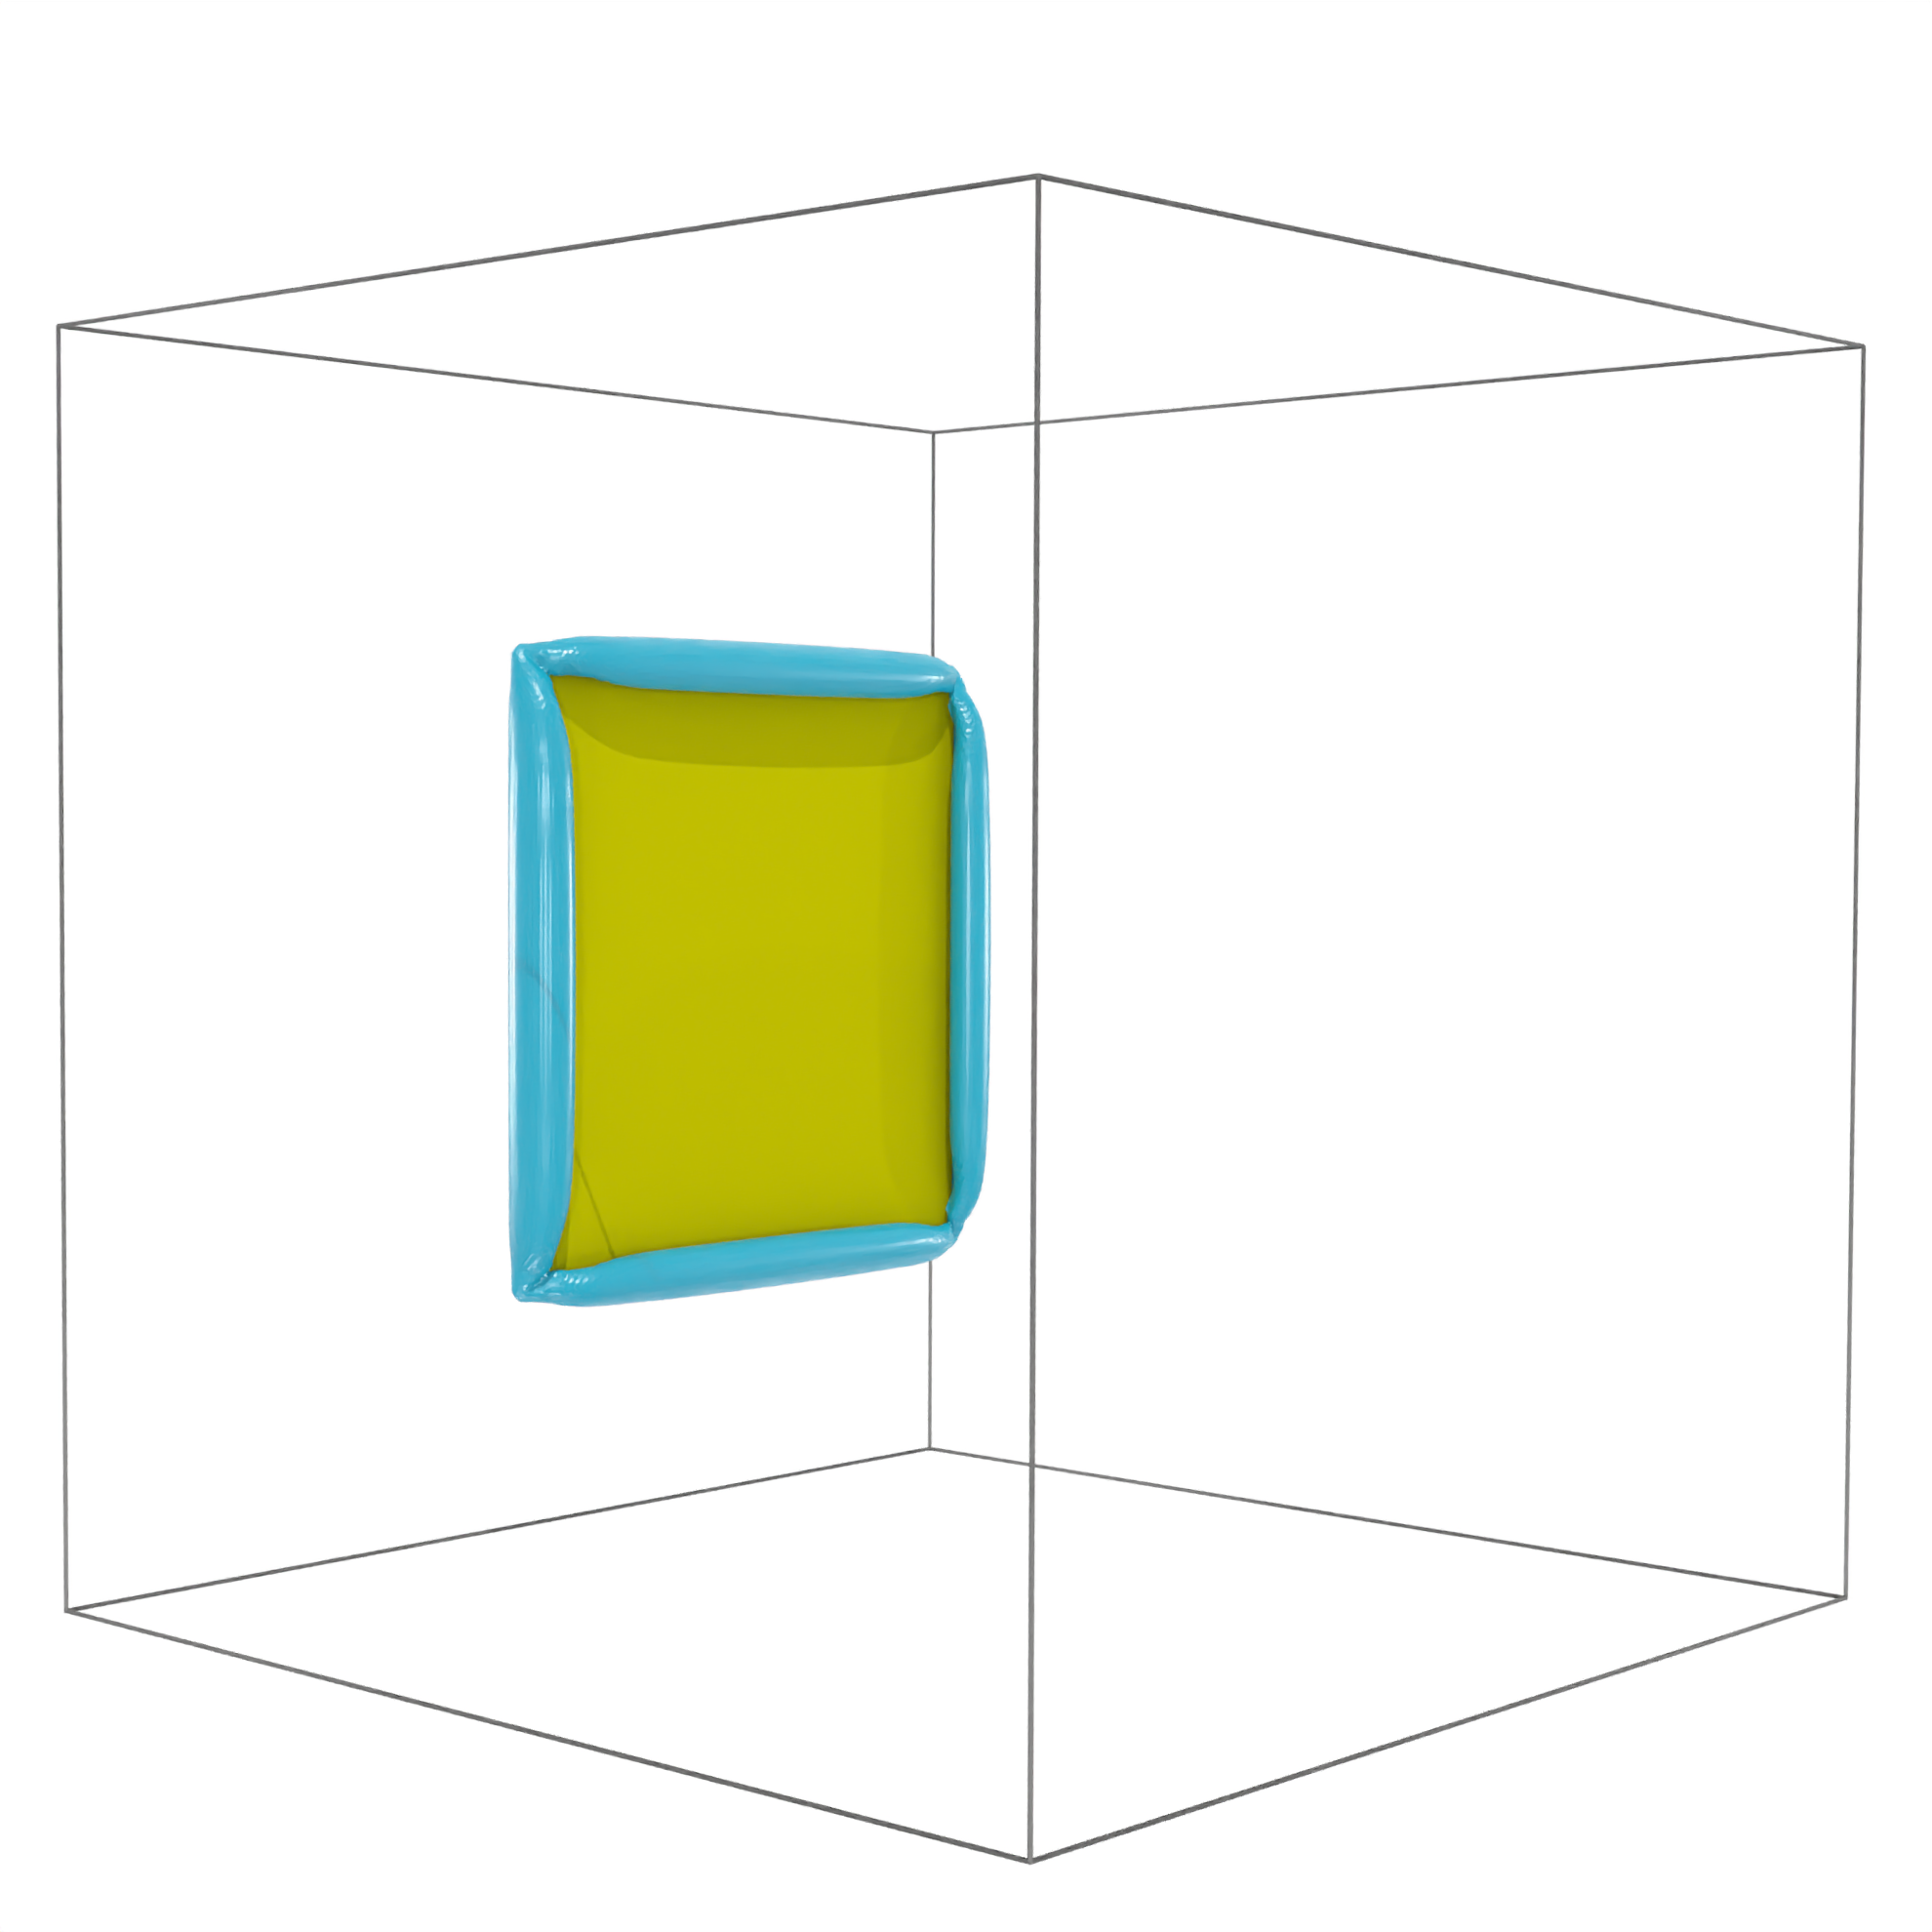
\includegraphics[width=\textwidth]{tex/fig/disk_high_re_2.png}
    \end{subfigure}%
    \begin{subfigure}{.33\textwidth}
        \centering
        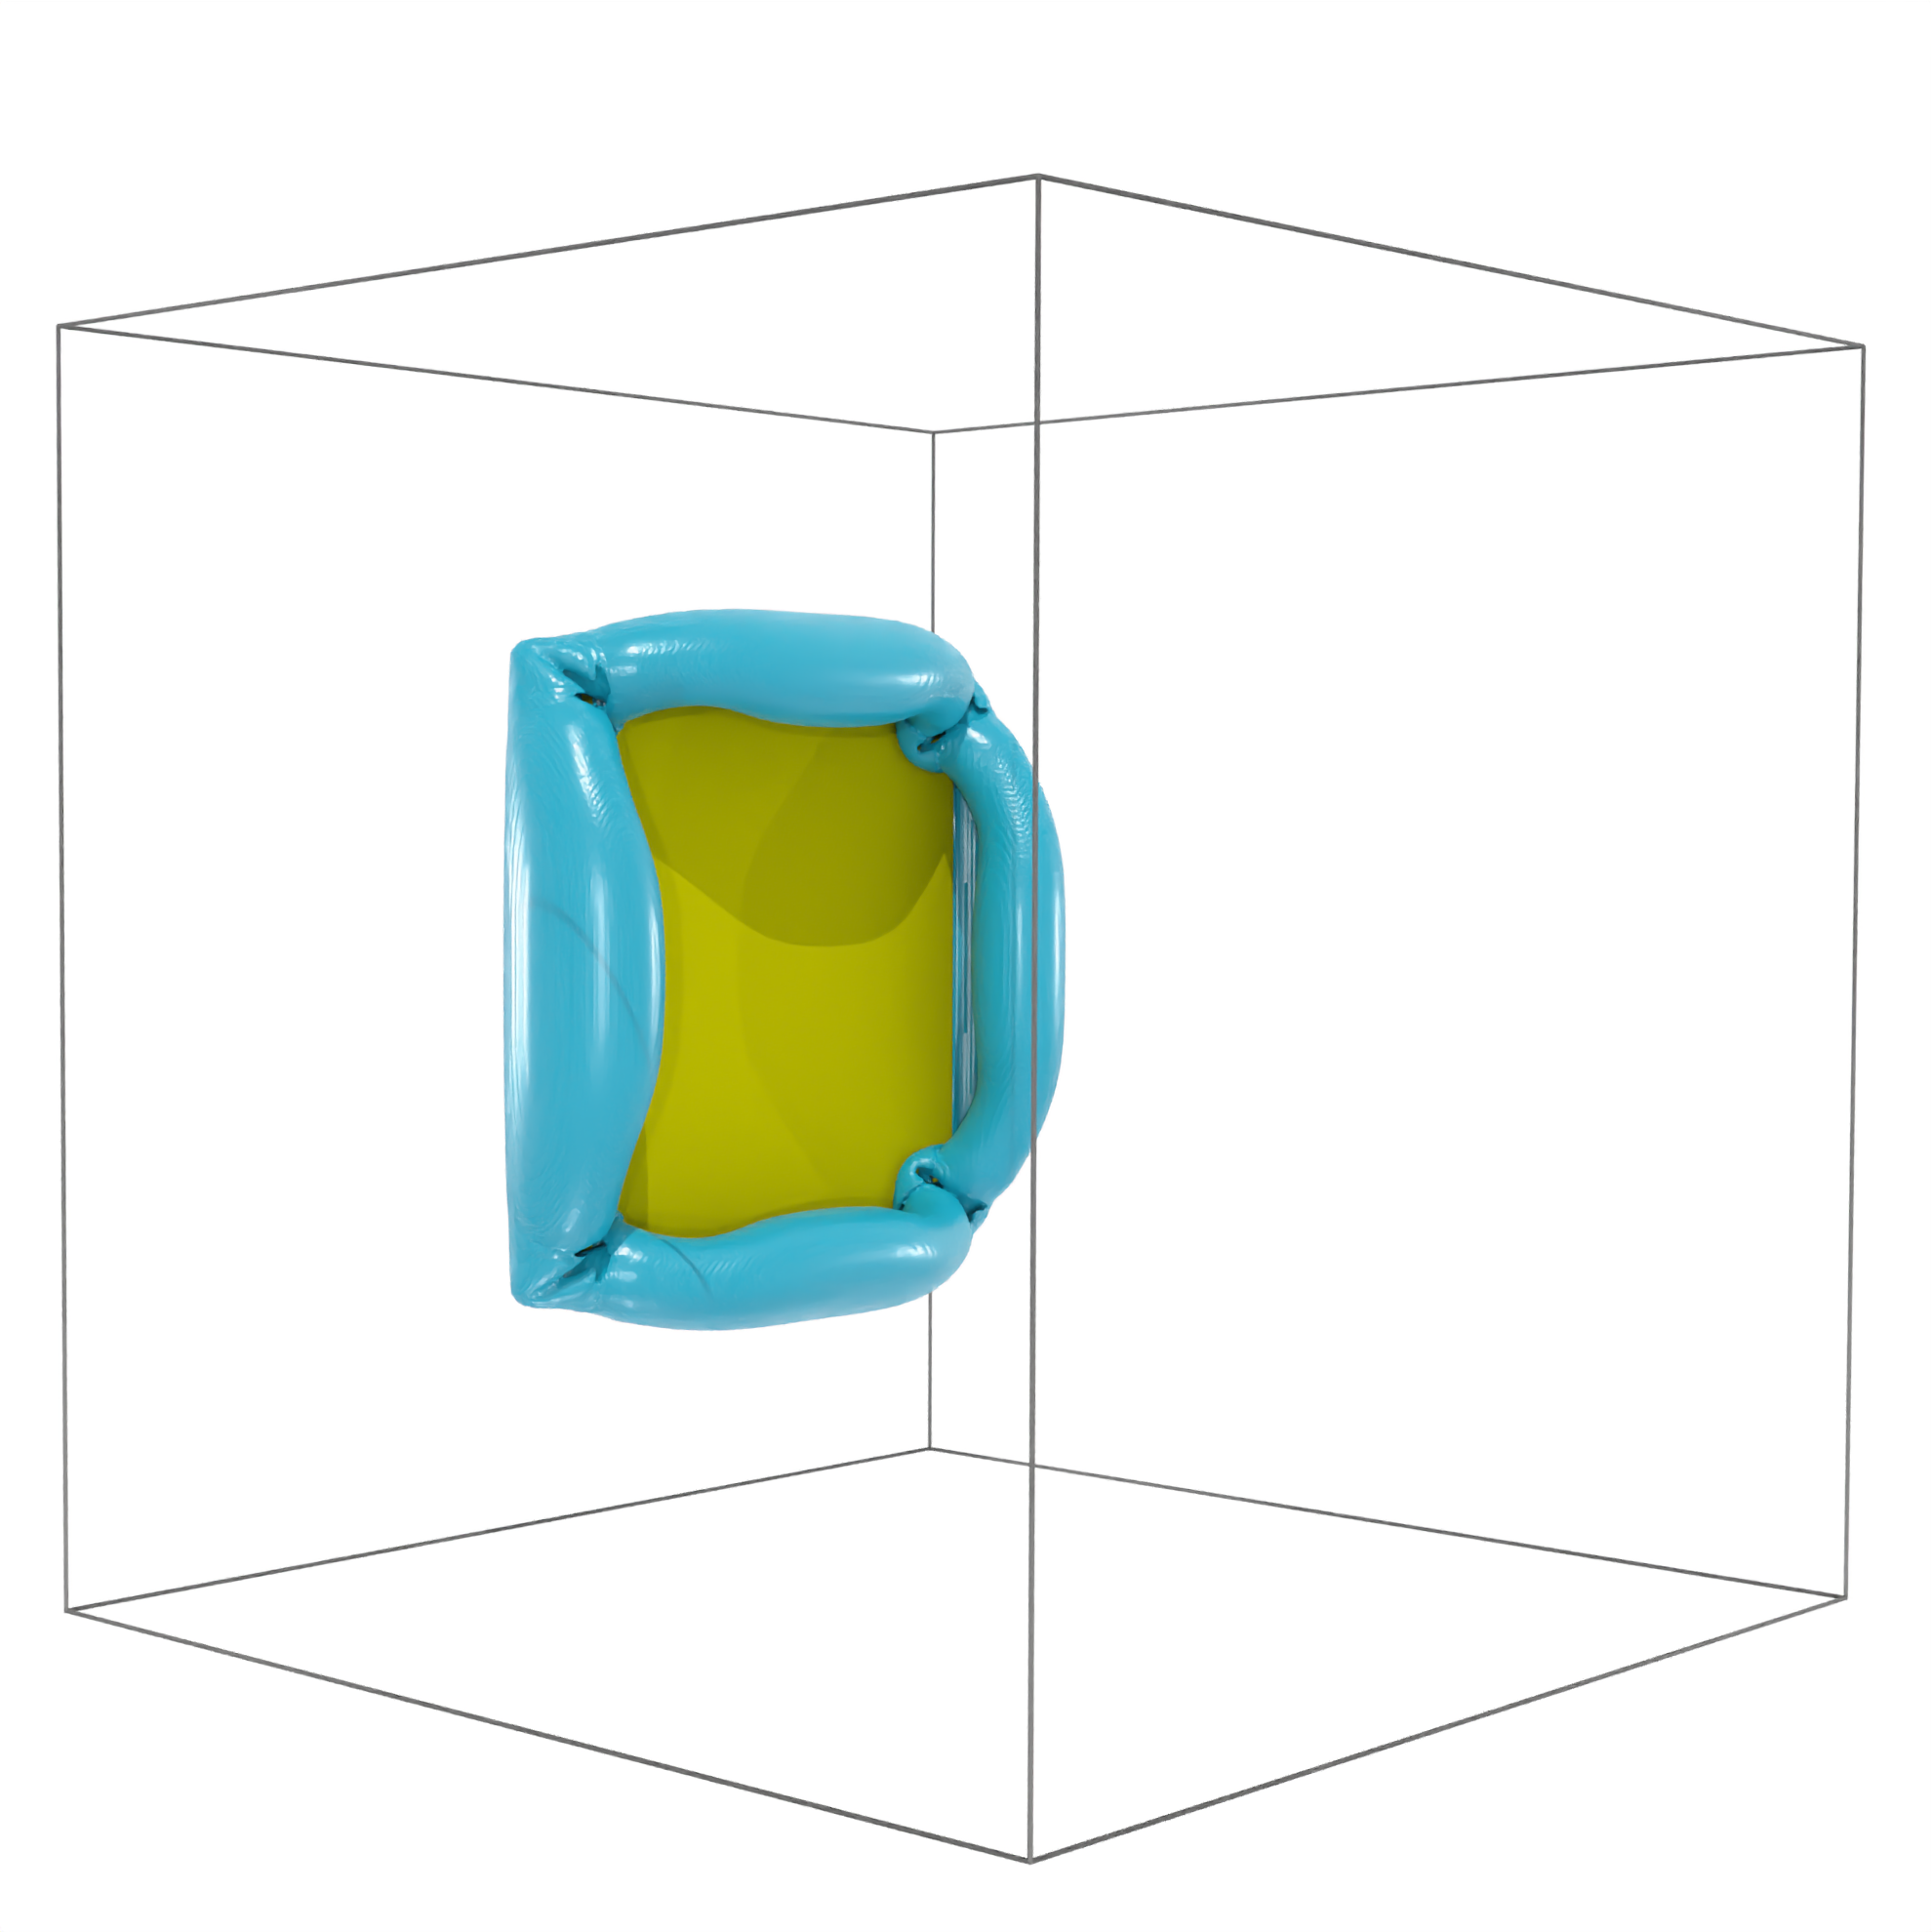
\includegraphics[width=\textwidth]{tex/fig/disk_high_re_3.png}
    \end{subfigure}%
    \begin{subfigure}{.33\textwidth}
        \centering
        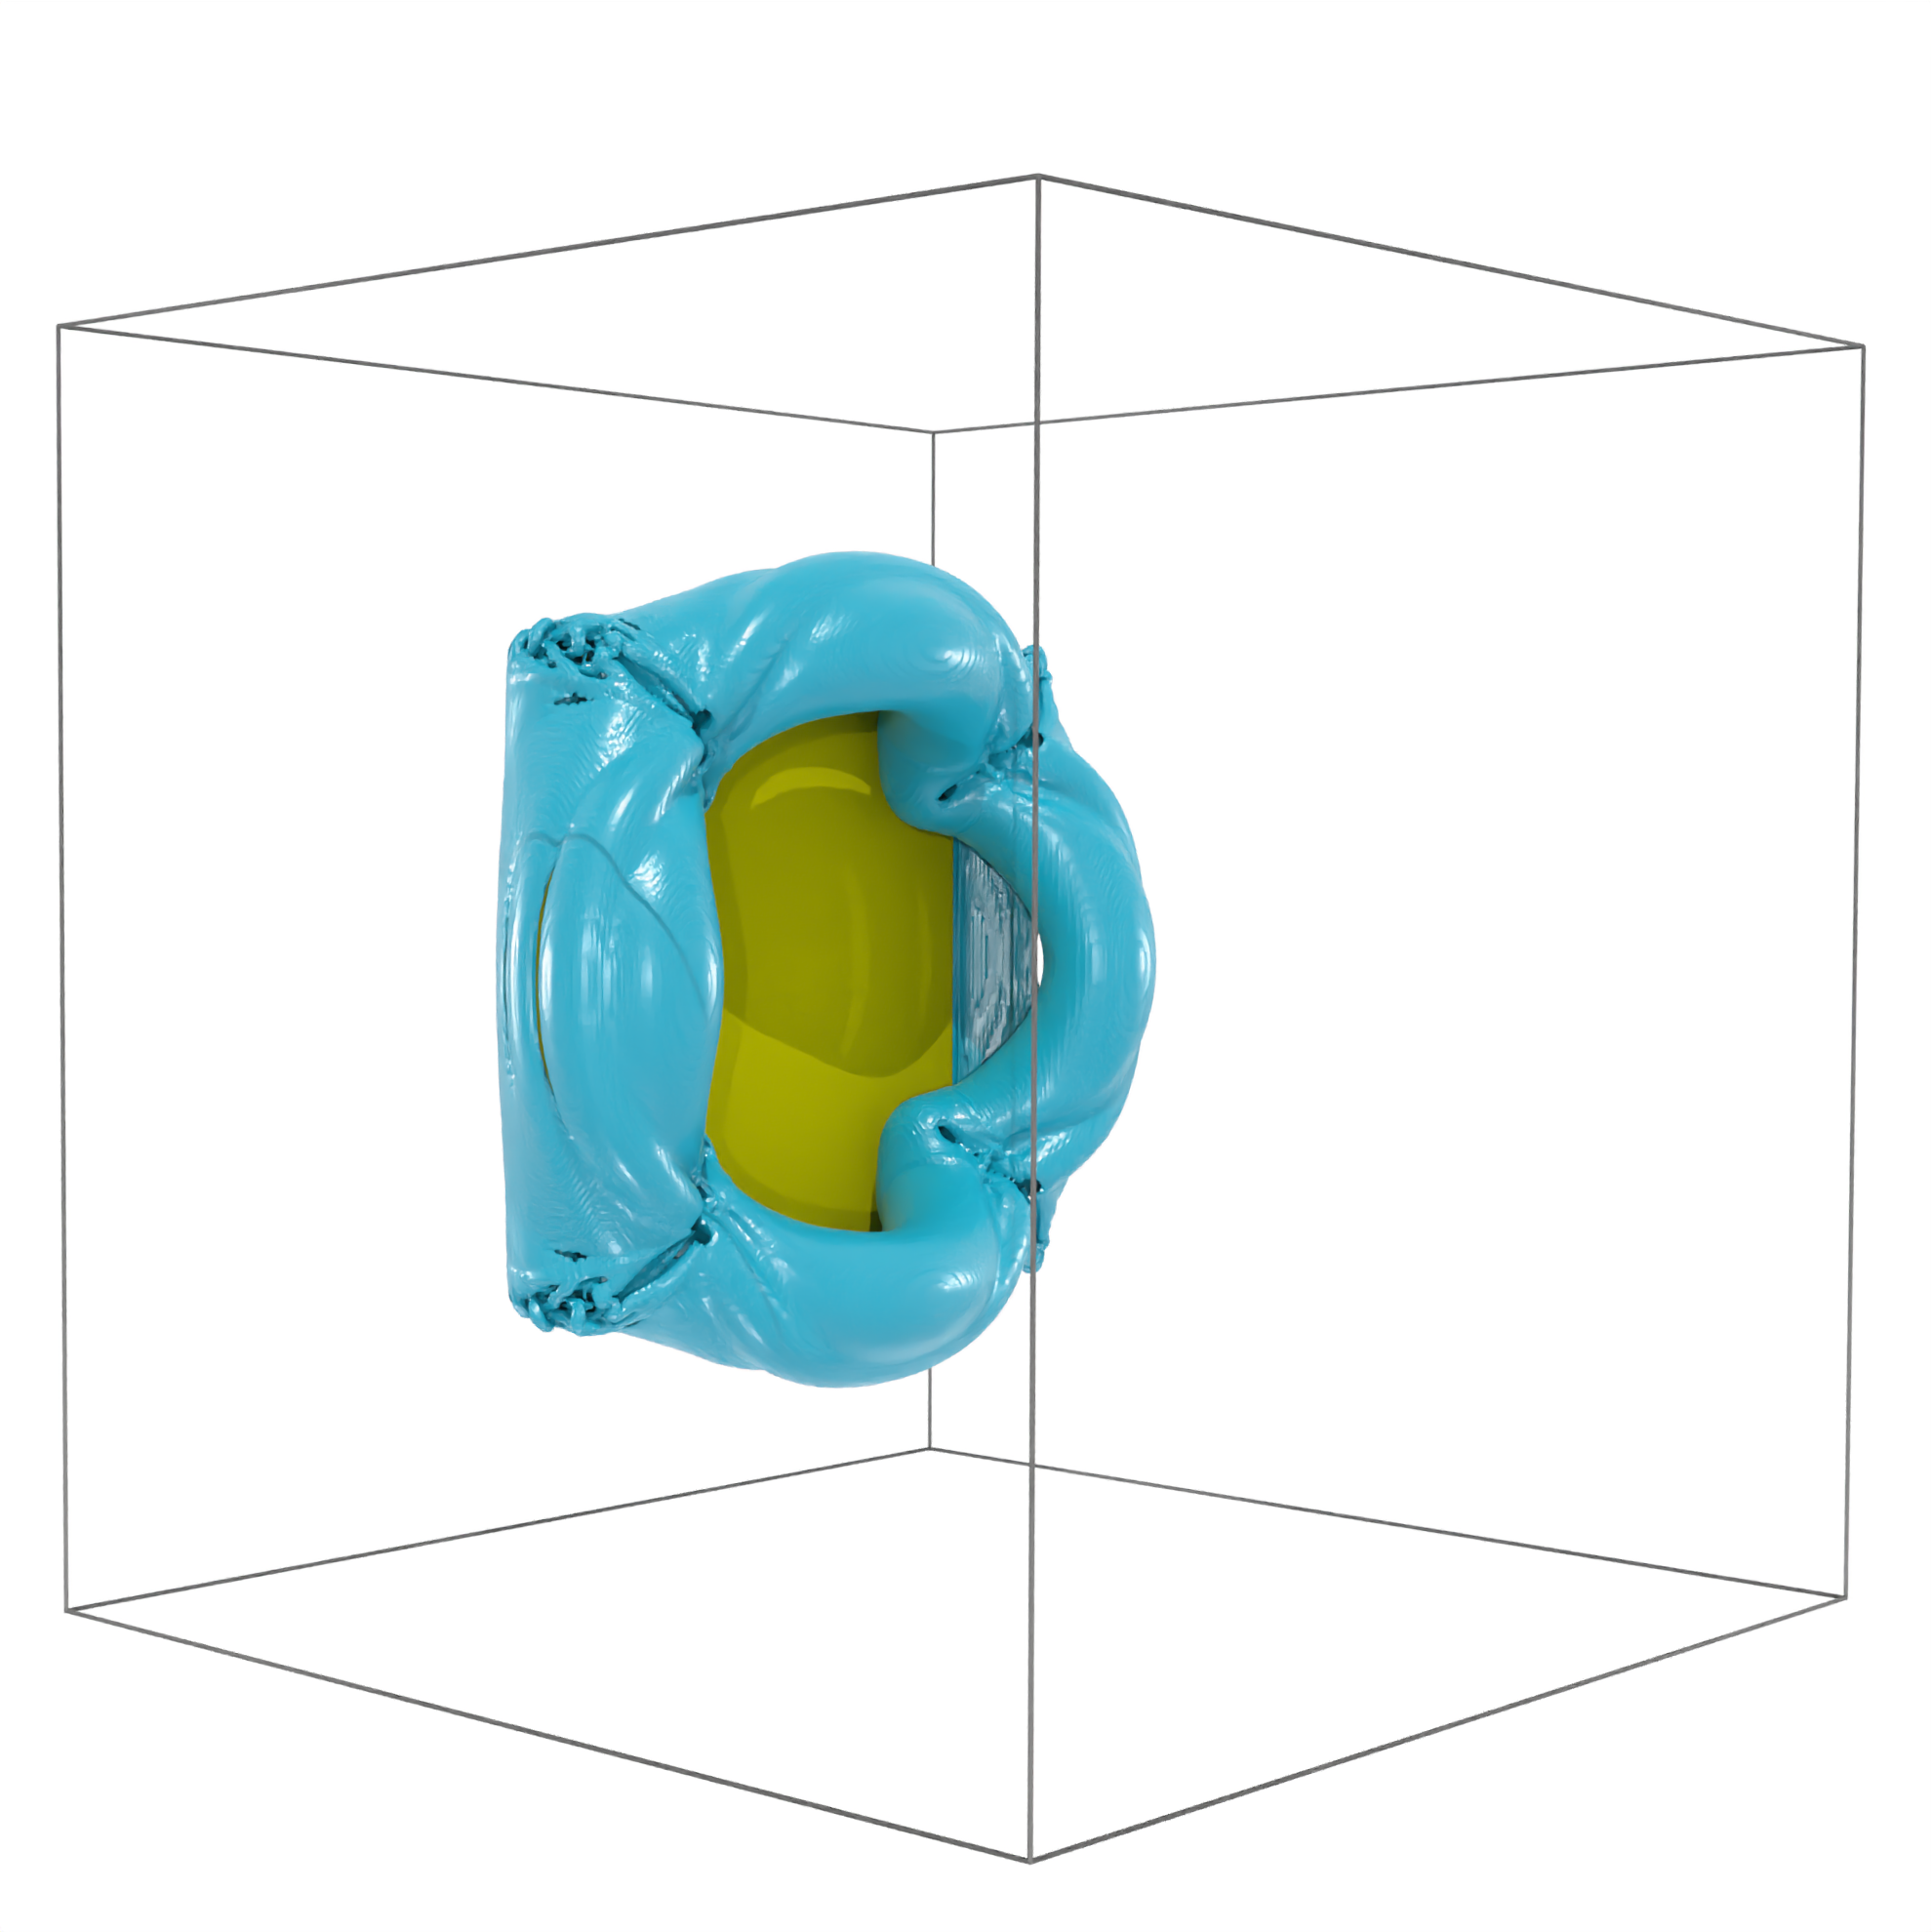
\includegraphics[width=\textwidth]{tex/fig/disk_high_re_4.png}
    \end{subfigure}
    \begin{subfigure}{.33\textwidth}
        \centering
        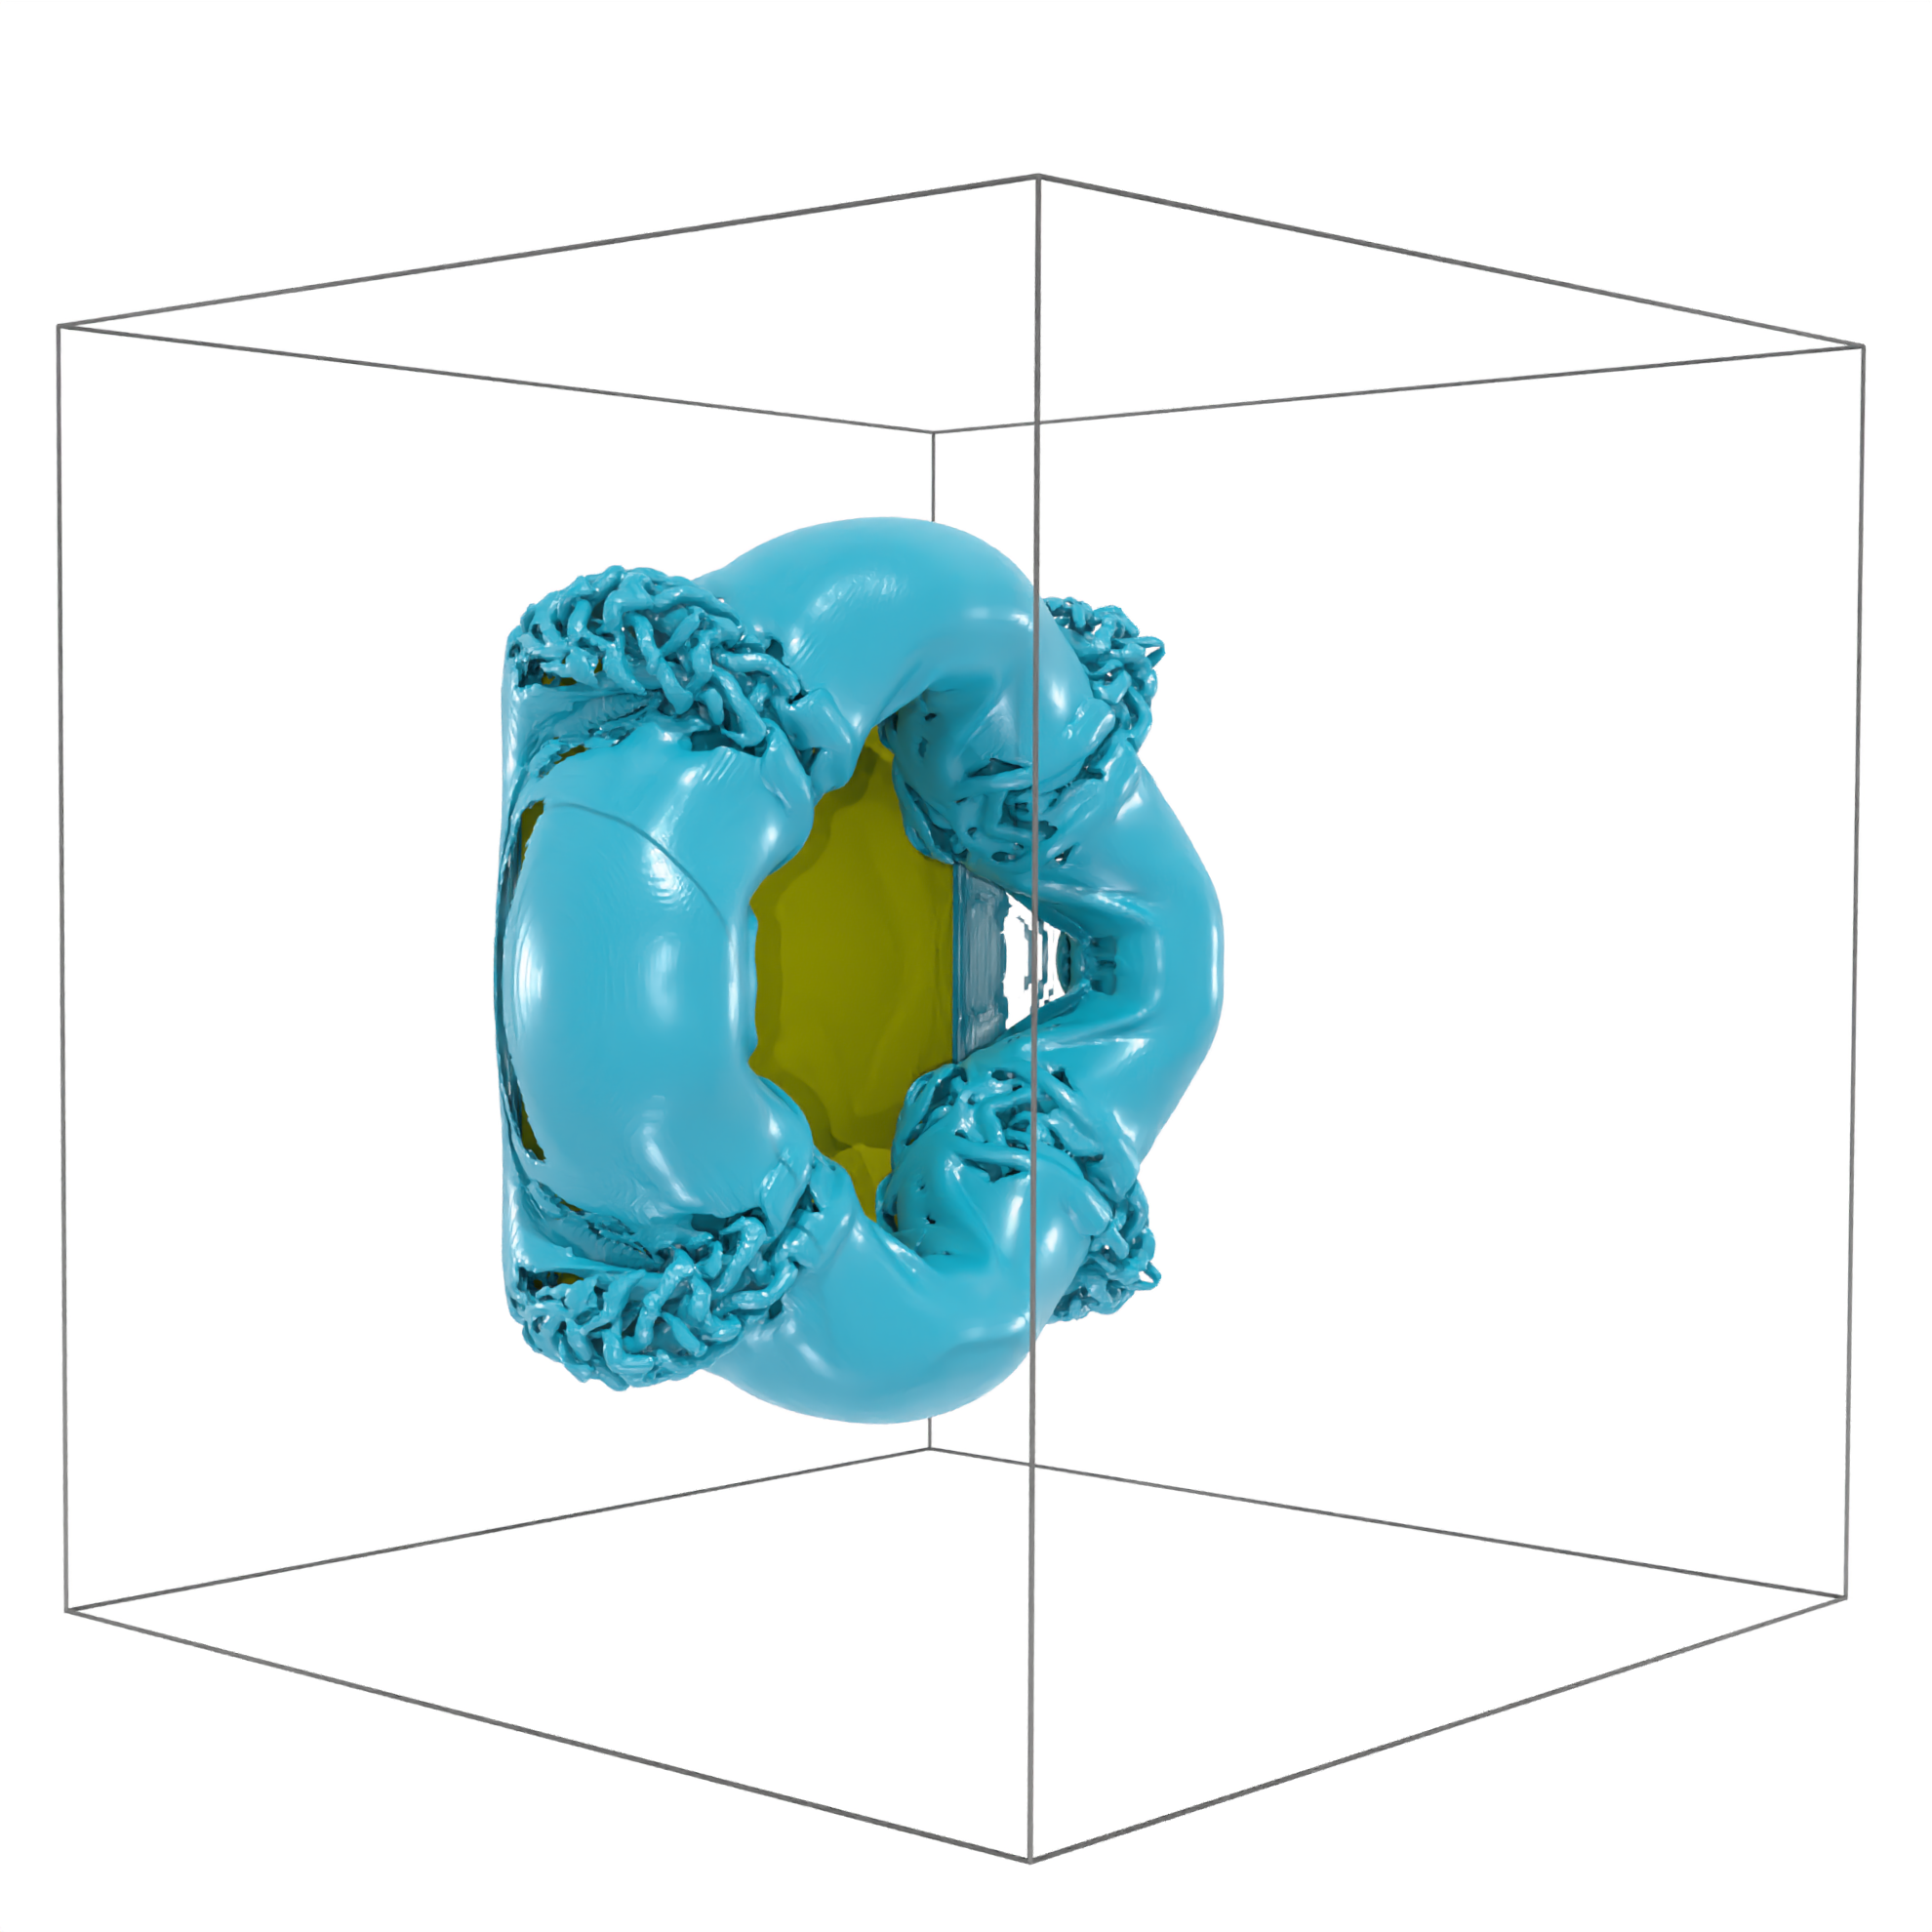
\includegraphics[width=\textwidth]{tex/fig/disk_high_re_5.png}
    \end{subfigure}%
    \begin{subfigure}{.33\textwidth}
        \centering
        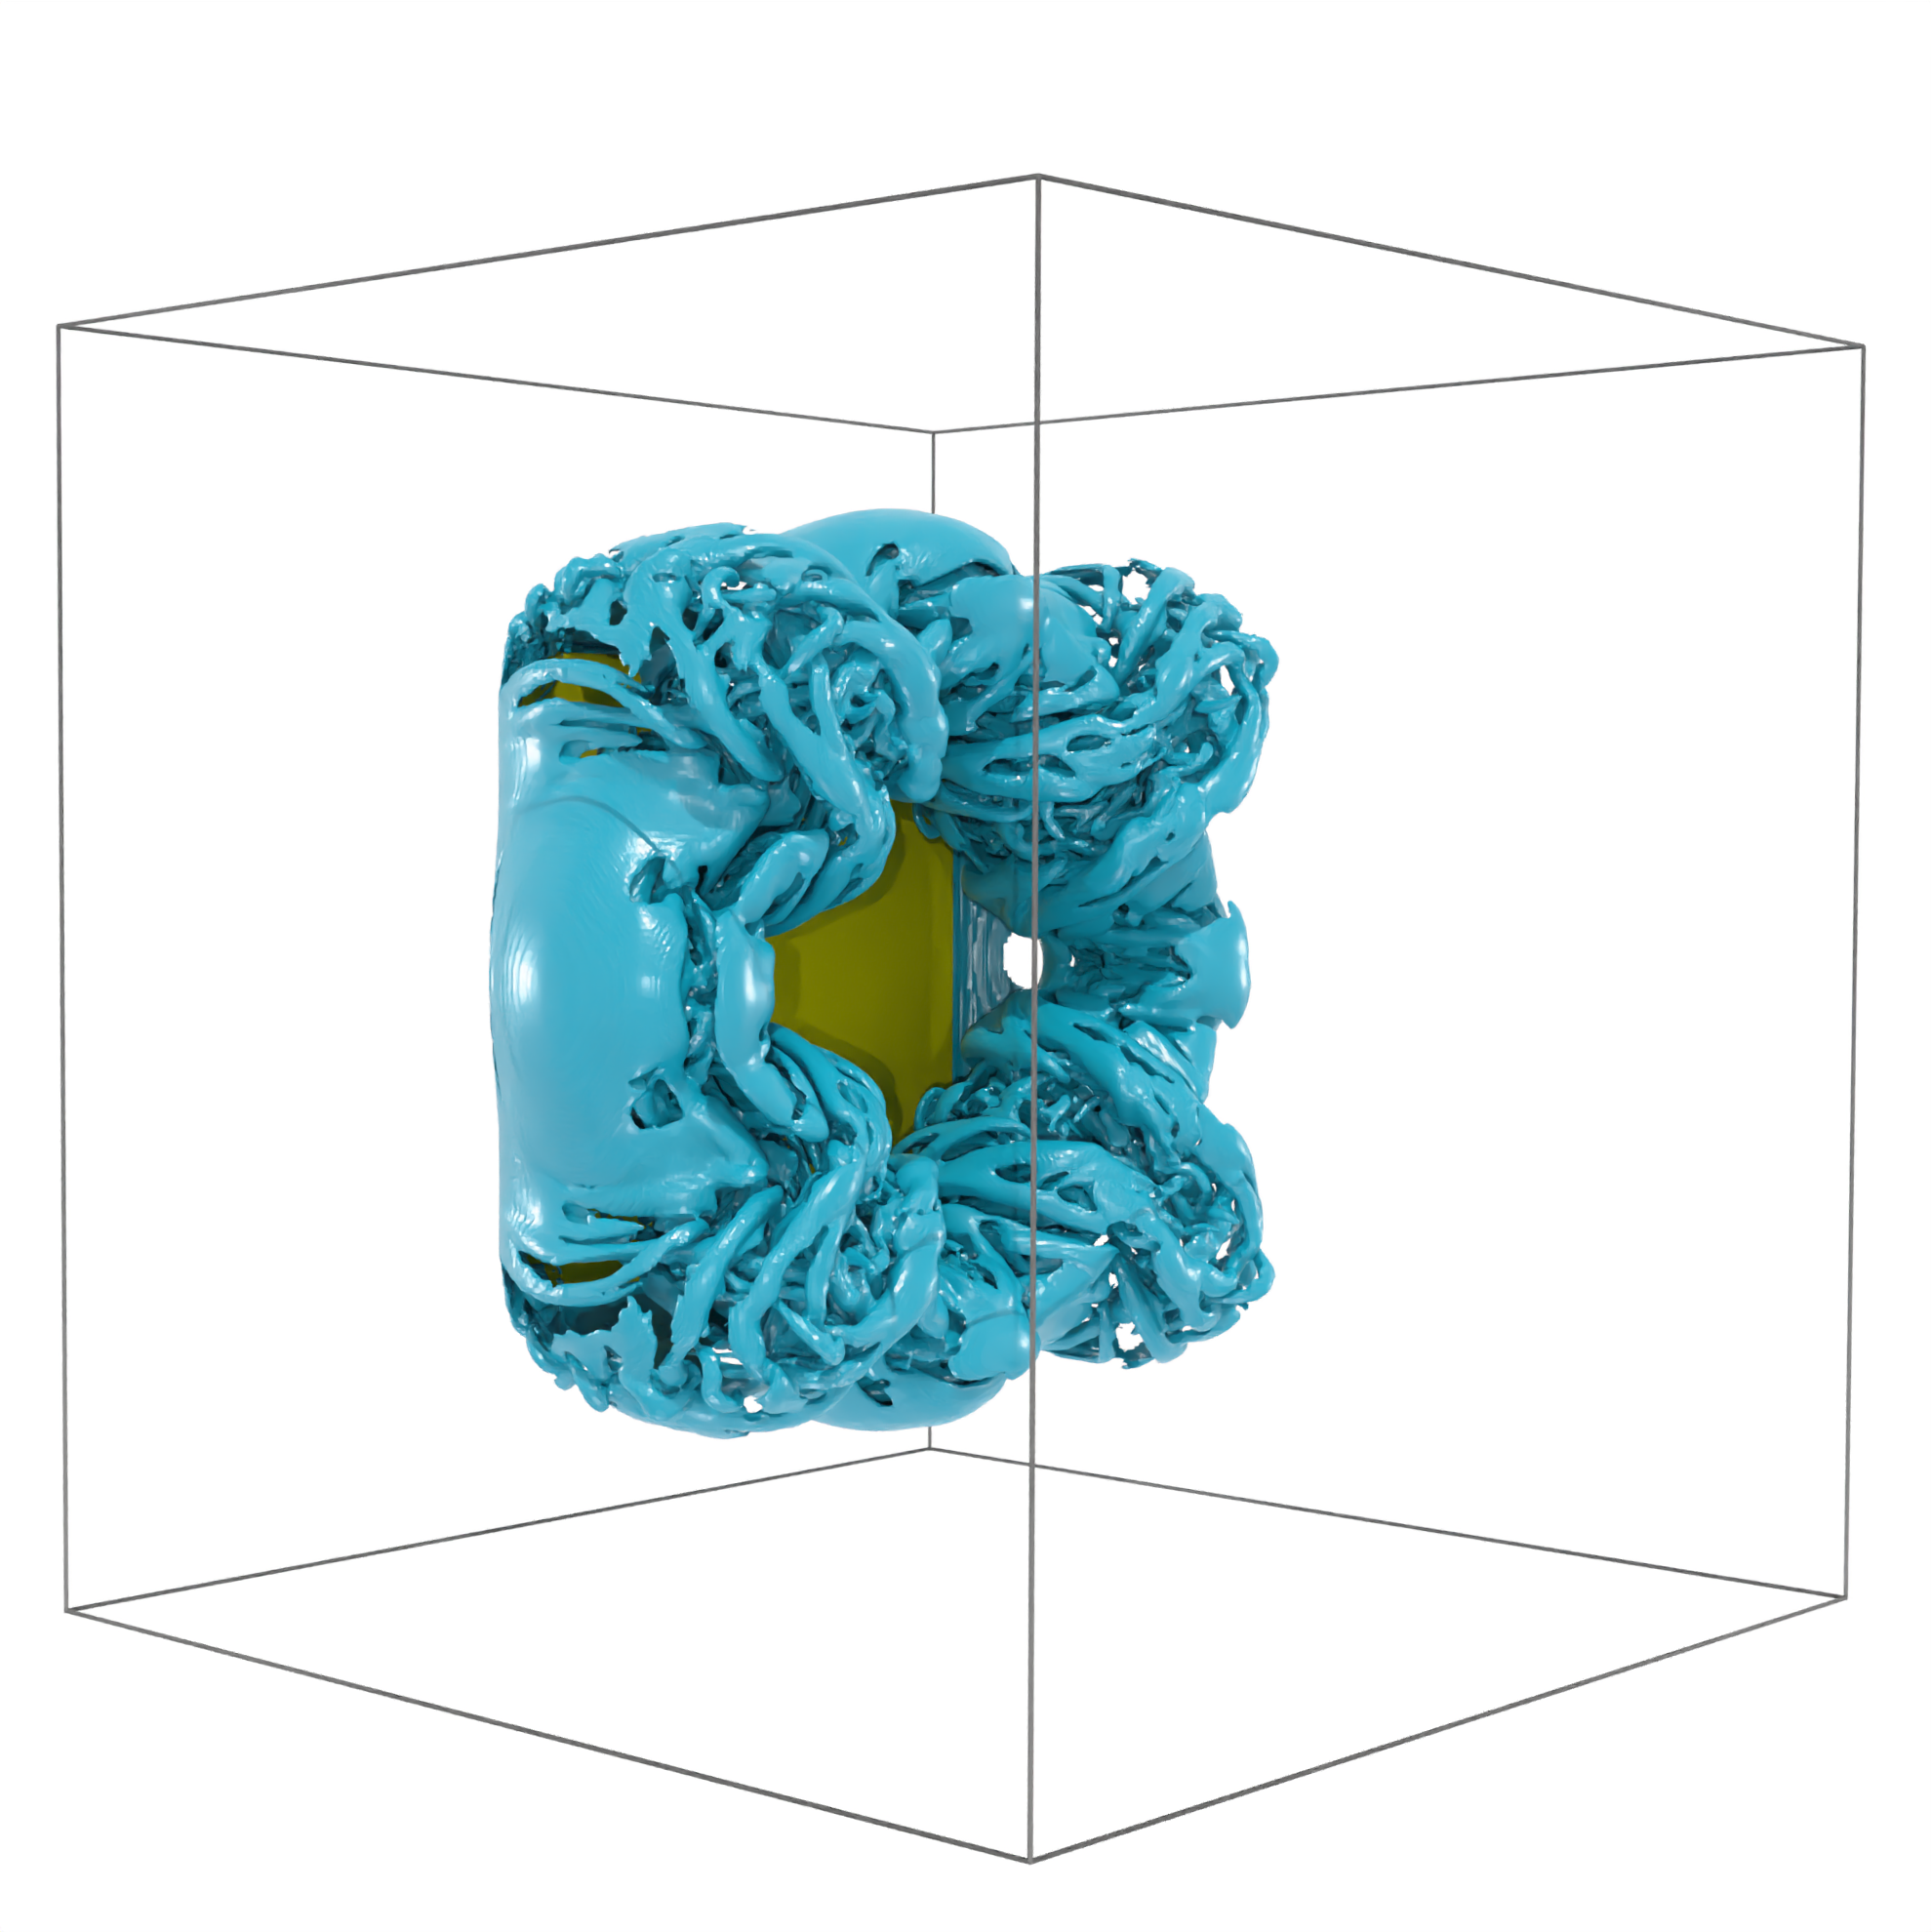
\includegraphics[width=\textwidth]{tex/fig/disk_high_re_6.png}
    \end{subfigure}%
    \begin{subfigure}{.33\textwidth}
        \centering
        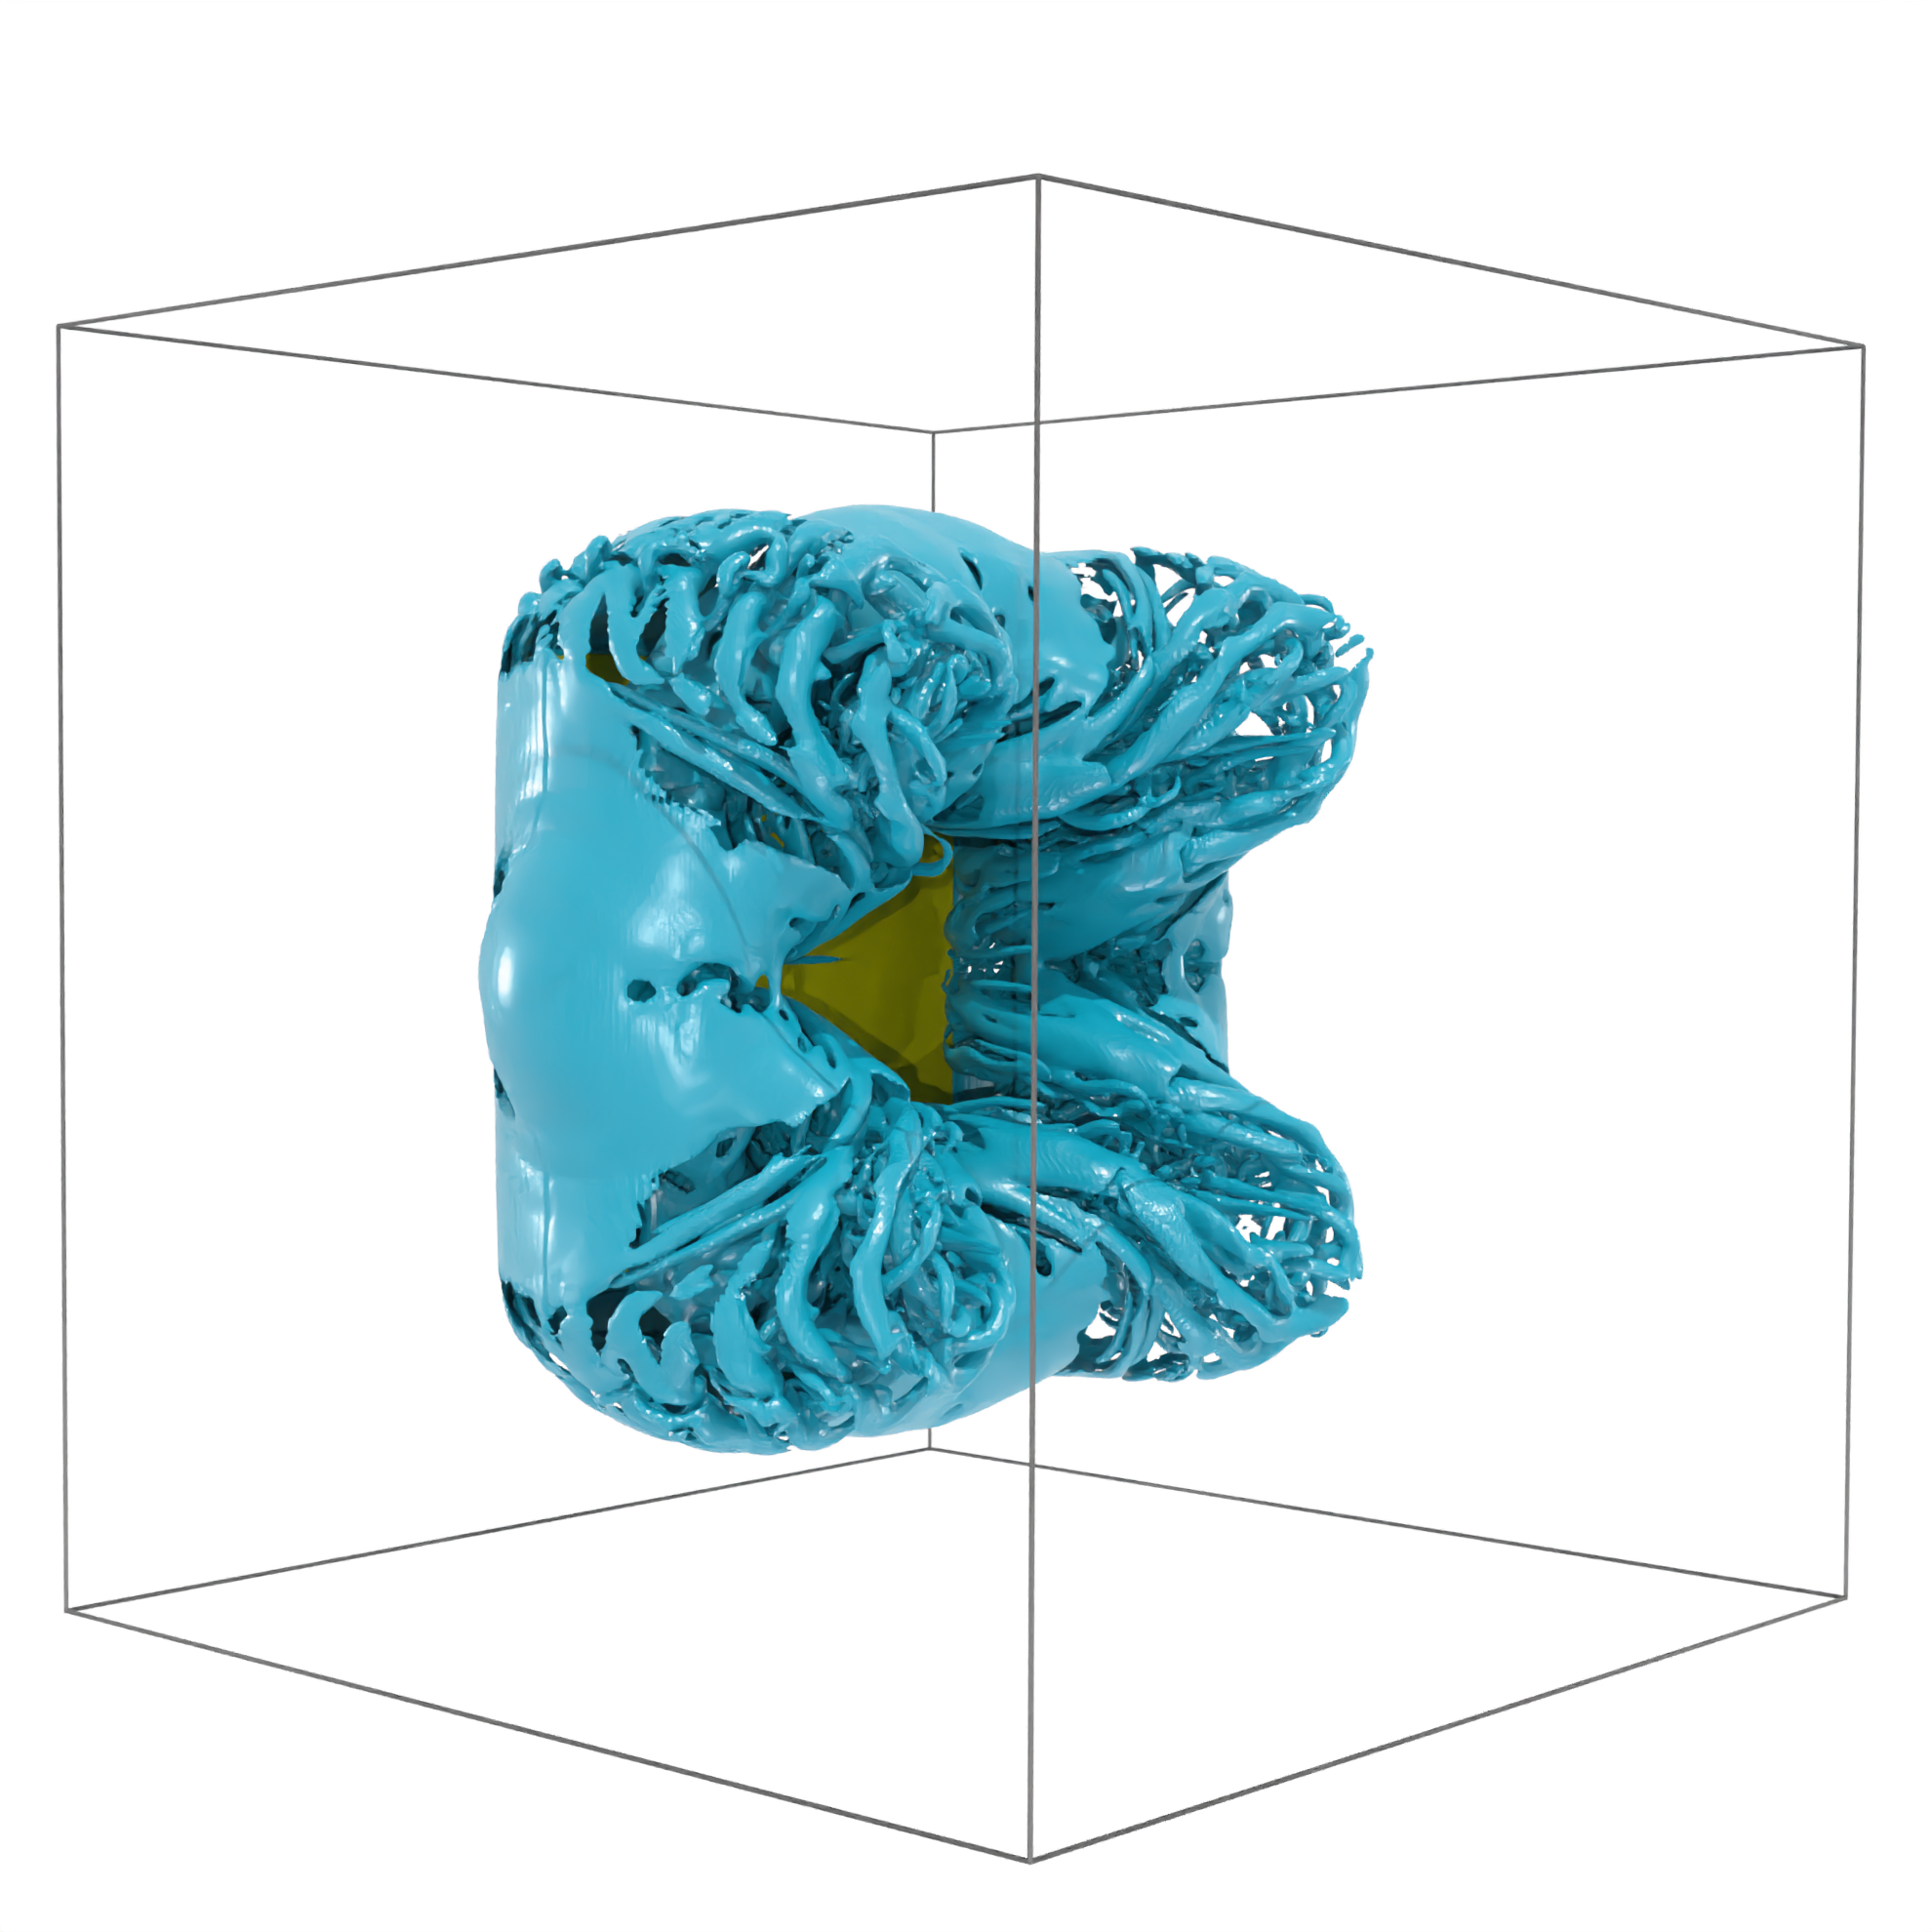
\includegraphics[width=\textwidth]{tex/fig/disk_high_re_7.png}
    \end{subfigure}
    \caption{Isocontour of $\lambda_2$-criterion $\lambda_2U^2/L^2=...$ for the flow around an initially stationary square plate at $Re=125\,000$ accelerated from rest in a quiescent flow at 6 convective times, $t^*\in [1,2,3,4,5,6]$, using the \emph{Biot-Savart} boundary conditions. The black frame represents the entire computational domain of size ($2L\times2L\times2L$)}
    \label{fig:disk_flow_3}
\end{figure}

Figure~\ref{fig:disk_flow_3} shows the vorticity generated by this accelerating body as six convective times $t^*\in[1,2,3,4,5,6]$. The vortices generated are shown via the $\lambda_2$-criterion \cite{JEong1995OnVortex}. The initial impulse generates a strong shear layer around the plate's edge that induces a strong vortex. Although the platform of the plate is square, this initial vortex rearrange itself into a shape resembling that of a vortex ring. After this initial vortex has traveled downstream, the plate's corner starts shedding smaller vortices that later trigger the breakdown of the start vortex. An animation of these still frames is provided in the supplementary material.

\section{Vortex-street applications}

Numerous examples of external flow violate our initial assumption that the vorticity is confined near the immersed body, far from the domain's boundary. We use two classical examples of vortex-street flows to investigate the effect of our short computational domain on flow history. First, the flow around a 2D cylinder at a Reynolds number $Re=200$, which results in the classical \emph{van K\`arm\`an} wake. Then, the reversed \emph{van K\`arm\`an} (or propulsive) wake generated by a heaving airfoil in a uniform flow at a range of Strouhal numbers.

\subsection{Flow around a 2D cylinder at $Re=200$}

We start our analysis with the flow behind a 2D circular cylinder of diameter $D$. The cylinder is immersed in a viscous fluid with free-stream velocity $U=(1,0)$. The viscosity is set such that the Reynolds number is $Re=\frac{UD}{\nu}=200$. We perform a domain study by varying the domain sizes from $5D\times3D$ up to $30D\times24D$ and, for each domain, compare the reflective and \emph{Biot-Savart} boundary conditions.

Figure.~\ref{fig:} flow vis

Figure~\ref{fig:cylinder_force} shows the total drag force acting on the cylinder for the various domain sizes and boundary conditions. The different domain sizes and the \emph{Biot-Savart} boundary conditions yield the best results with an excellent collapse of the drag forces, regardless of the domain size. Simulations performed with the \emph{Biot-Savart} boundary conditions are insensitive to domain size. Reflective boundary conditions induce extremely large blockage effects for small domains and only slowly converge to the \emph{Biot-Savart} boundary solution for significantly larger domains.

We note here that the computational time for the smaller domain that uses the \emph{Biot-Savart} boundary conditions is equivalent to that of \textbf{add computational time}. However, the convergence of the results with domain size is far superior.

In addition to the total drag forces acting on the cylinder, we look at the vortex shedding frequency in the wake. Here again, the \emph{Biot-Savart} boundary conditions show an excellent collapse of the shedding frequency, which matches that of classical bluff body vortex shedding frequency of $St\sim 0.3$ \cite{}. The high blockage effect induced by the reflective boundary conditions induces fast flow around the cylinder, increasing the shedding frequency to higher values with reflective boundary conditions.

\begin{figure}
    \centering
    \begin{subfigure}{.5\textwidth}
        \centering
        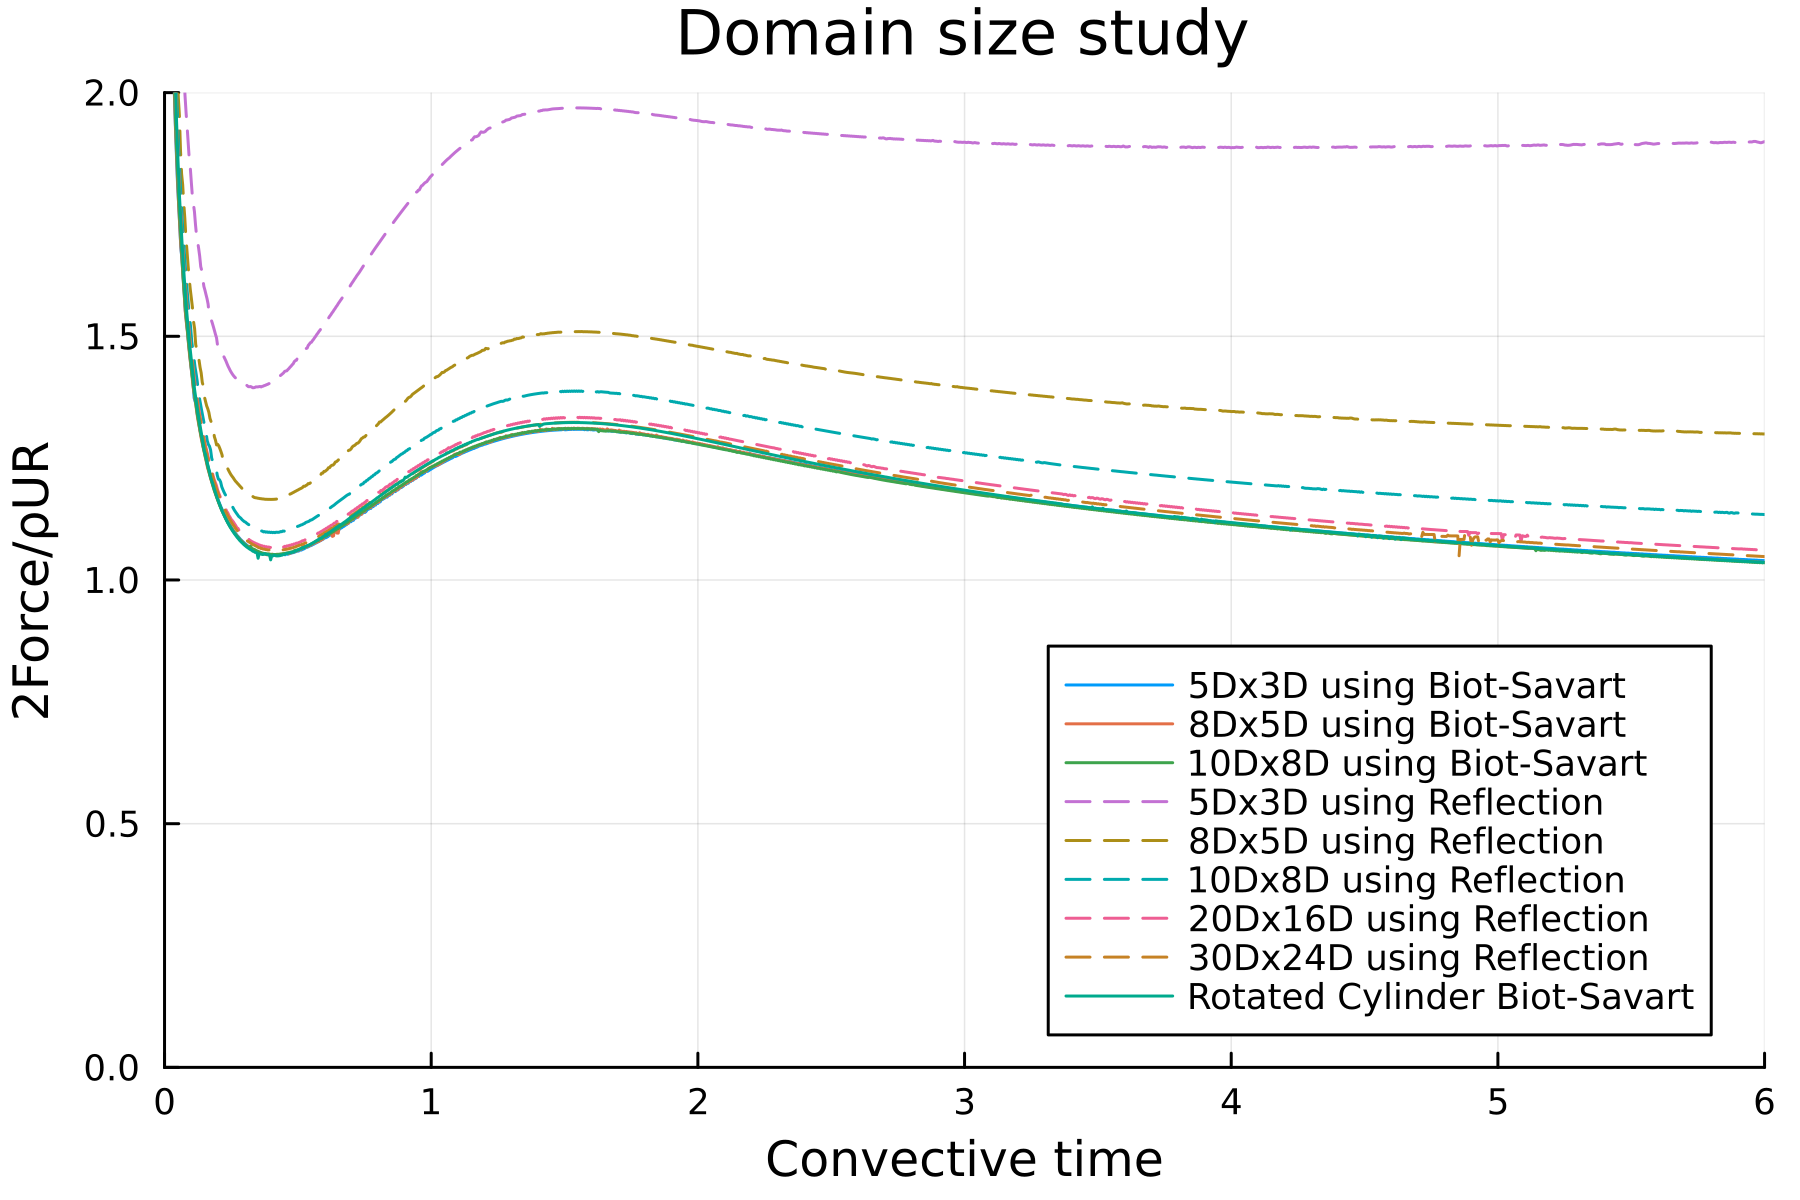
\includegraphics[width=\textwidth]{tex//fig/force.png}
    \end{subfigure}%
    \begin{subfigure}{.5\textwidth}
        \centering
        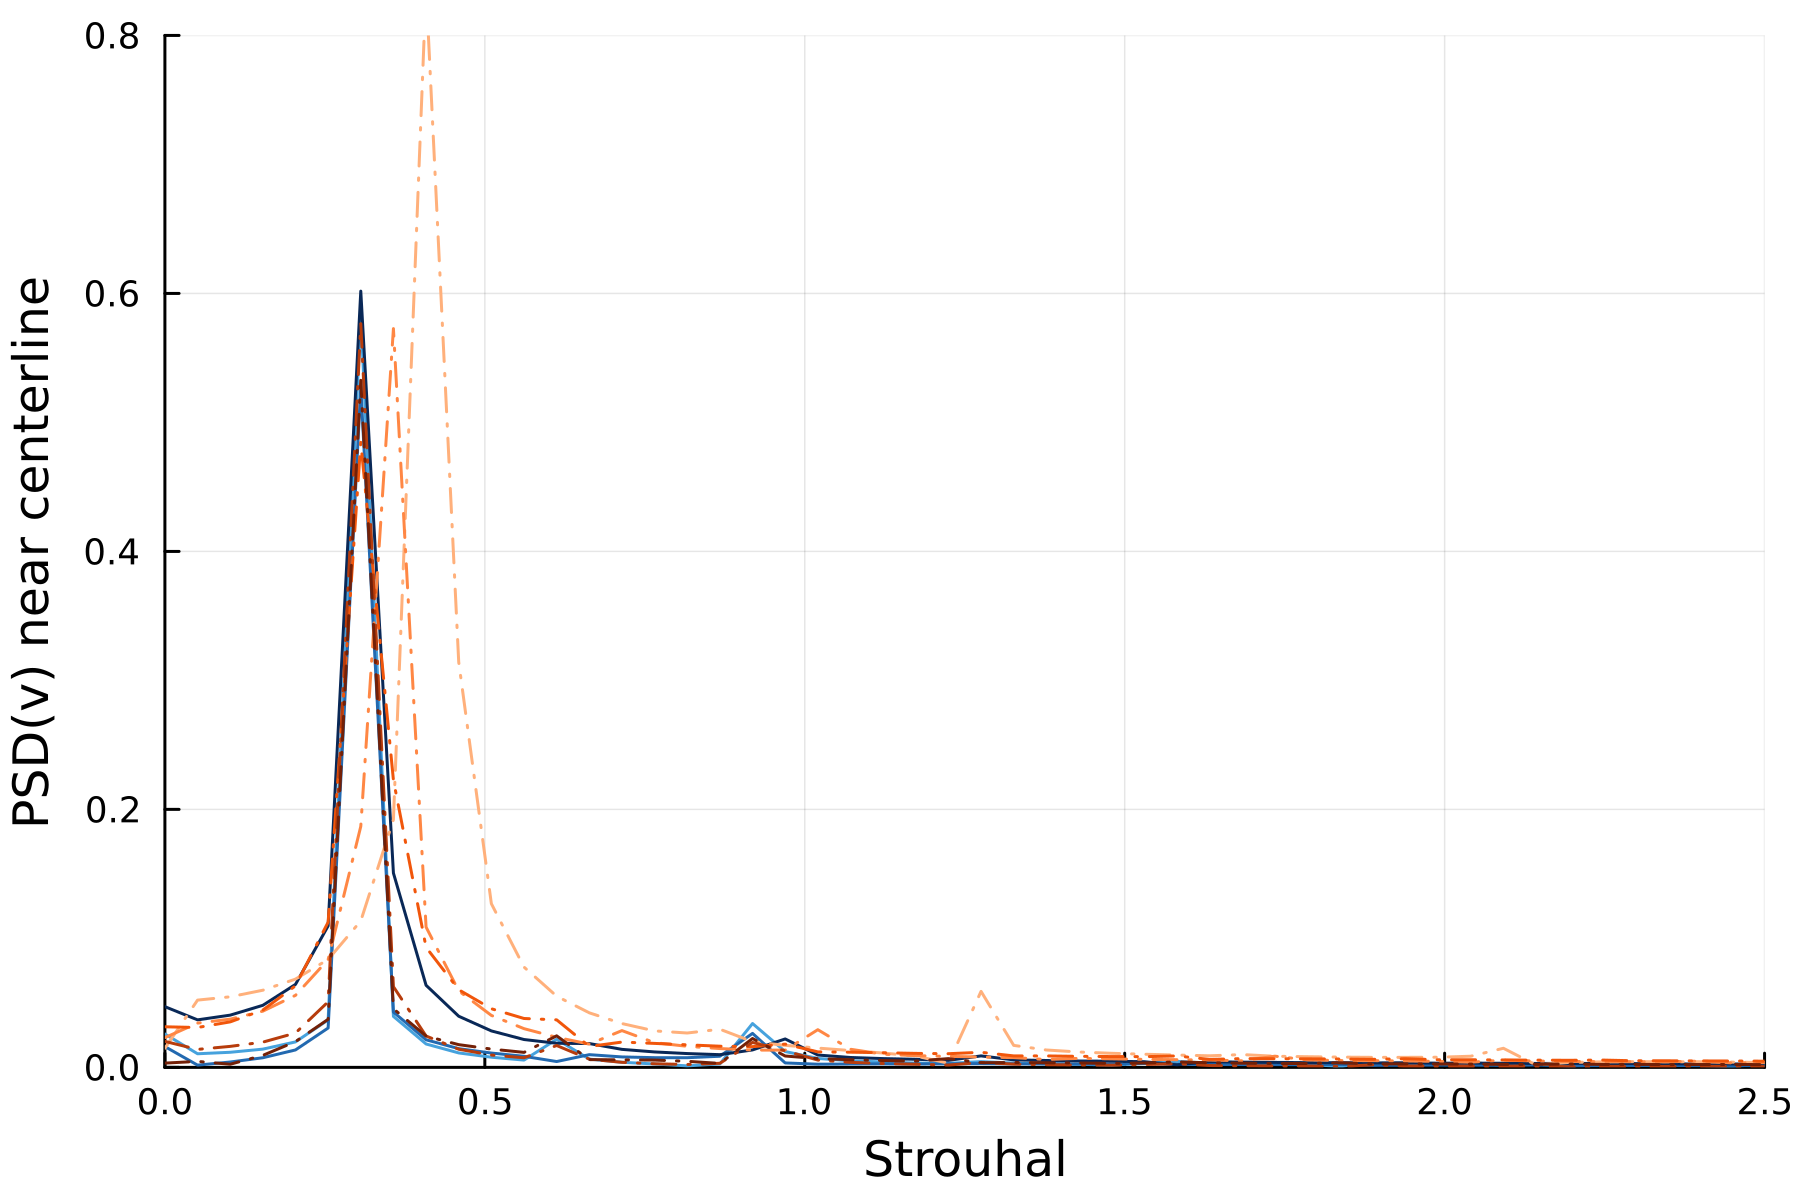
\includegraphics[width=\textwidth]{tex/fig/fft.png}
    \end{subfigure}%
    \caption{(left) Drag force acting on the circular cylinder at $Re=200$ for various combinations of boundary conditions and domain size. The rotated domain consists of a $4D\times4D$ domain, with the cylinder centered at $1.5D\times1.5D$ and a free stream velocity of $U=(1/\sqrt2,1/\sqrt2)$. (right) The frequency spectrum of the wake of the cylinder for the same combination of boundary conditions and domain size shows the classical shedding frequency at $St=0.3$.}
    \label{fig:cylinder_force}
\end{figure}

These results suggest that, for drag wake at least, the wake history on the immersed body is very small. However, propulsive systems use thrust wakes where wake history is expected to be higher.

\subsection{Wake behind a heaving foil}

We continue our analysis with thrust wakes. We immerse a rigid foil of length $L$ moving with a linear velocity $\vec{U}=(U,0)$ in a viscous fluid. In addition to it's steady forward speed, the foil undergoes a pure heave motion of amplitude $h_0$
\begin{equation}
    y(t) = h_0 \sin(2\pi f t)
\end{equation}
where $h_0/L=0.5$ is the non-dimensional amplitude, and the frequency is $f = St\,U/h_0$. For Strouhal number $St<0.5$, the airfoil generates thrust, and almost no net lift, and for $St>0.6$, the wake generated by this flapping foil is strongly asymmetric and generates a significant net lift force. We perform simulations of this system for a range of Strouhal numbers and compare the mean lift force and wake obtained on a large domain ($30L\times20L$) with standard reflective boundary conditions to the ones obtained on two different domains of size ($6L\times4L$) and ($12L\times8L$) that use the \emph{Biot-Savart} boundary conditions. We simulate the flow around this heaving airfoil for 100 convective times to ensure that the wake stabilizes, and we gather pressure and viscous forces for the last 20 convective times. Mean lift forces are obtained by time-averaging these forces over the past 20 convective times.

For $St<0.5$, we observe almost no difference between the different boundary conditions and domain sizes. The wake is symmetric, and the airfoil produces zero mean lift forces; see Fig.~\ref{fig:deflected_wake_2}. For $St\ge 0.5$ we start to observe wake deflection on the large domains with the reflective boundary condition.

\begin{figure}
    \centering
    \begin{subfigure}{.48\textwidth}
        \centering
        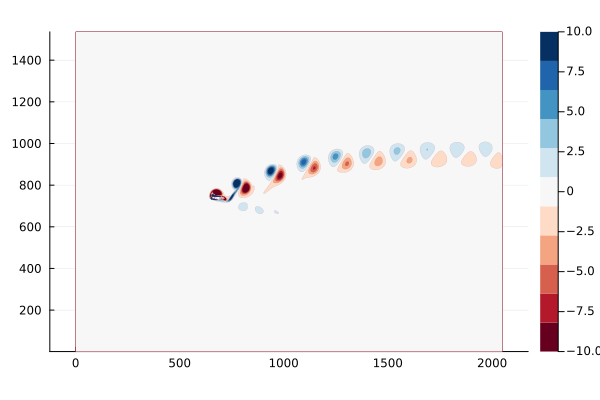
\includegraphics[trim={2.8cm 2cm 4cm 2cm},clip,width=\textwidth]{tex//fig/Deflected_wake_snap.png}
        \caption{Reflection ($30L\times20L$)}
    \end{subfigure}%
    \hspace{0.1cm}
    \begin{subfigure}{.48\textwidth}
        \centering
        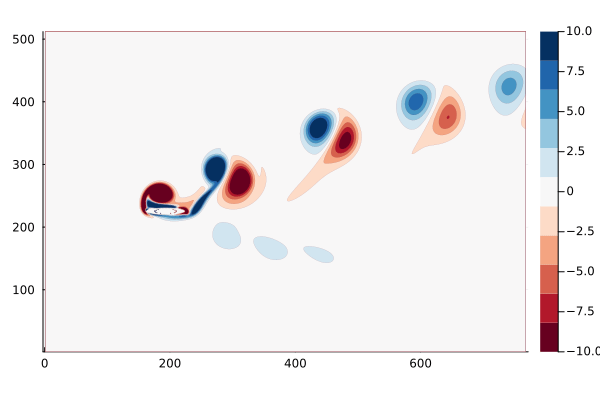
\includegraphics[trim={2.8cm 2cm 4cm 2cm},clip,width=\textwidth]{tex/fig/Deflected_wake_snap_small.png}
        \caption{Reflection - near wake}
    \end{subfigure}
    \begin{subfigure}{.48\textwidth}
        \centering
        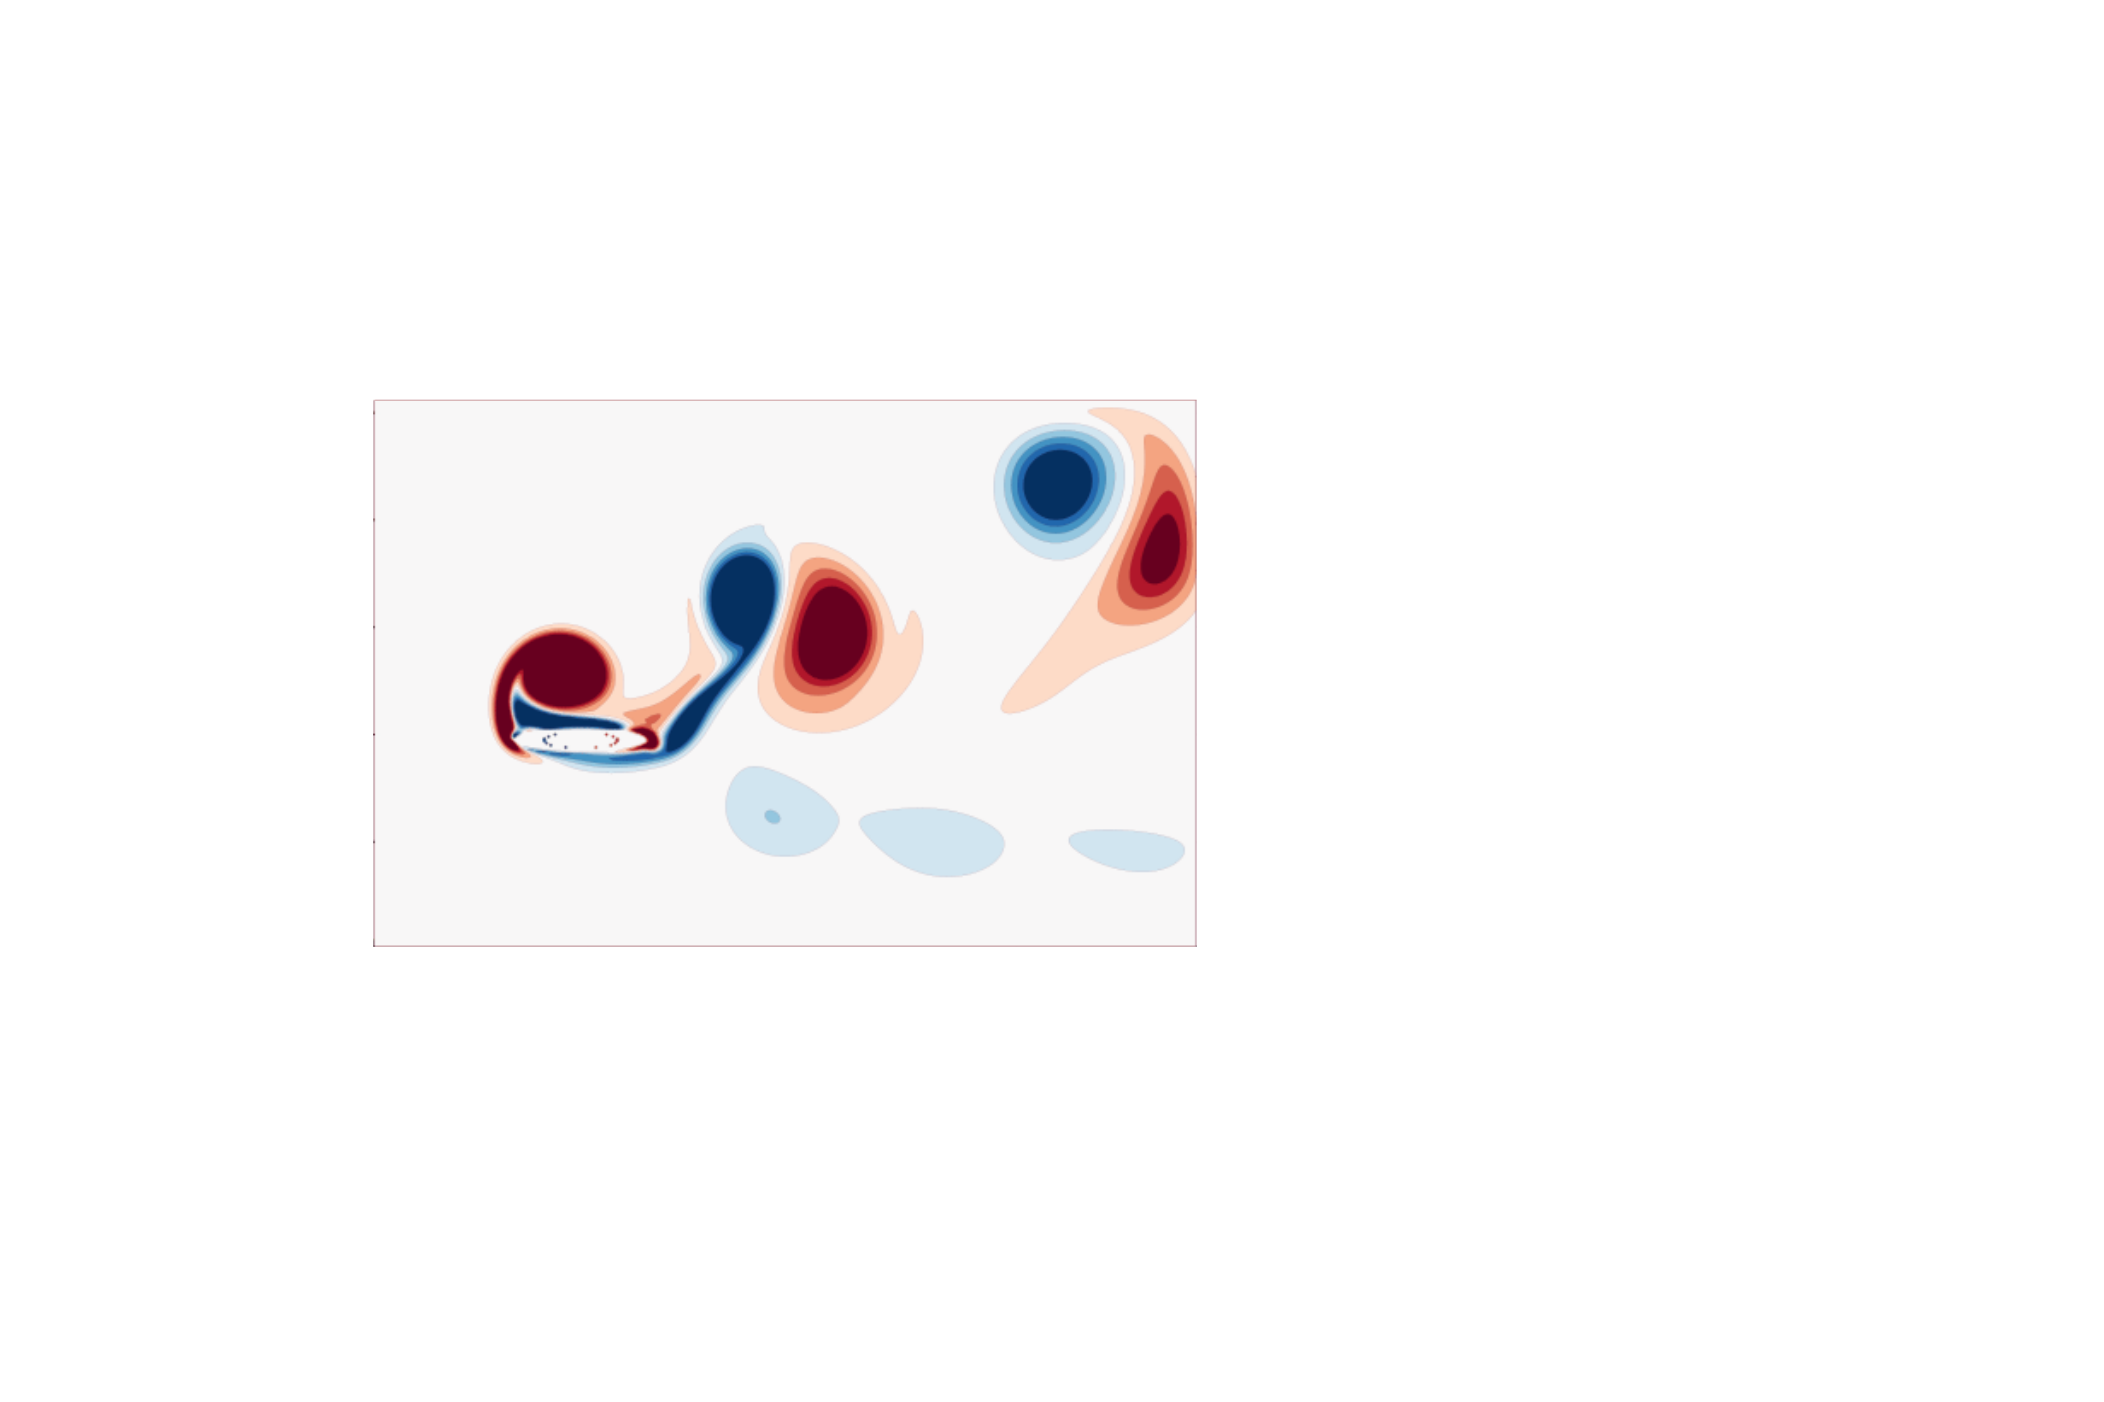
\includegraphics[trim={2.8cm 2cm 4cm 2cm},clip,width=\textwidth]{tex//fig/Deflected_wake_snap_BS.png}
        \caption{\emph{Biot-Savart} ($6L\times4L$)}
    \end{subfigure}%
    \hspace{0.1cm}
    \begin{subfigure}{.48\textwidth}
        \centering
        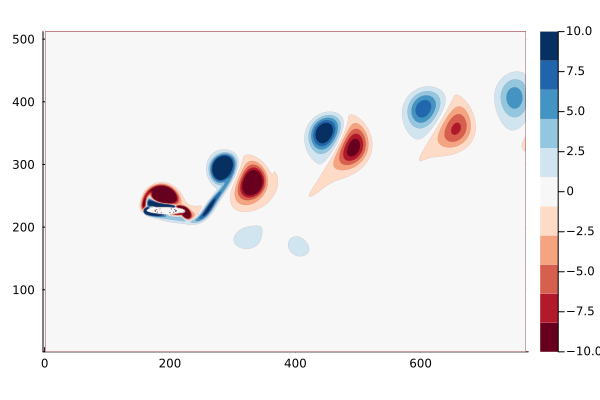
\includegraphics[trim={2.8cm 2cm 4cm 2cm},clip,width=\textwidth]{tex//fig/Deflected_wake_snap_BS_2x.png}
        \caption{\emph{Biot Savart} ($12L\times8L$)}
    \end{subfigure}
    \caption{Snapshot of the deflected wake behind an airfoil at $St=0.6$ and $Re=100$ for an amplitude to chord ratio $h_0/L=1.0$. The upper left panel $(a)$ shows the far wake obtained with the reflective boundary condition in a large domain, the upper right panel $(b)$ shows a zoom onto the airfoil and the near wake, the bottom left $(c)$ panel shows the entire (small) \emph{Biot-Savart} domain used for the computation (the dashed line represents the domain boundaries) and the lower right panel $(d)$ shows the entire (larger) \emph{Biot-Savart} domain. Vorticity is shown as 10 equally spaced isocontours in the interval $\omega L/U \pm 10$.}
    \label{fig:deflected_wake}
\end{figure}

Fig.~\ref{fig:deflected_wake} shows the vorticity field generated by the wing at $St=0.6$. The left panel shows the complete wake obtained with the large domain of size ($30L\times20L$). The left panel is a zoomed-in version of the same simulation, using a field of view with the size of the largest \emph{Biot-Savart} domain. Finally, the bottom row shows two \emph{Biot-Savart} simulations with two different domain sizes. The left panel shows the smallest domain of size ($6L\times4L$), represented by the gray dashed line, and the right panel shows a larger domain of size ($12L\times8L$) which extends to the whole panel.

Wake history strongly influences the near wake; the large domain correctly captures this, and a strong wake deflection is observed (the first vortex shed sets the direction; in this case, it is shed in the negative $y$ direction).

\begin{figure}
    \centering
    \begin{subfigure}{.5\textwidth}
        \centering
        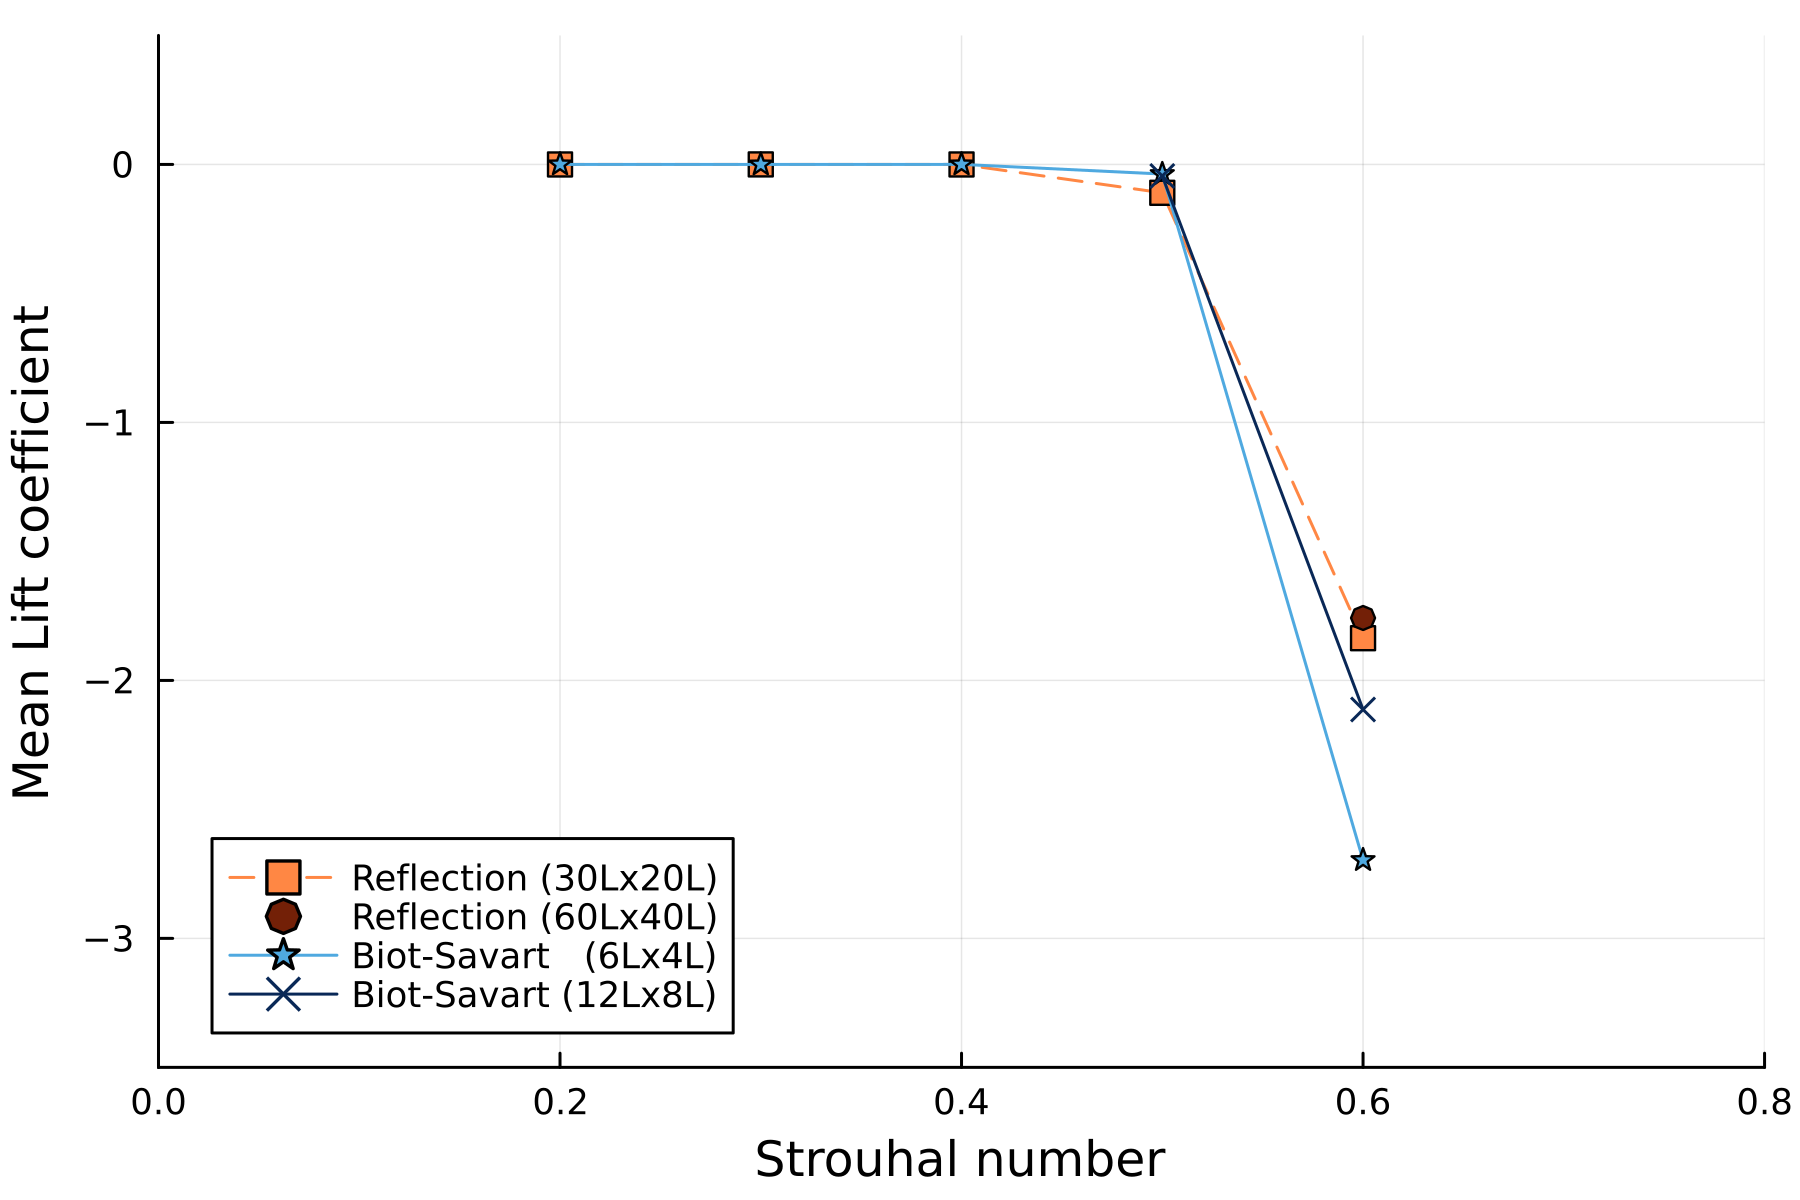
\includegraphics[trim={0 0 0 0},clip,width=\textwidth]{tex/fig/CL_mean_deflected_wake.png}
    \end{subfigure}%
    \begin{subfigure}{.5\textwidth}
        \centering
        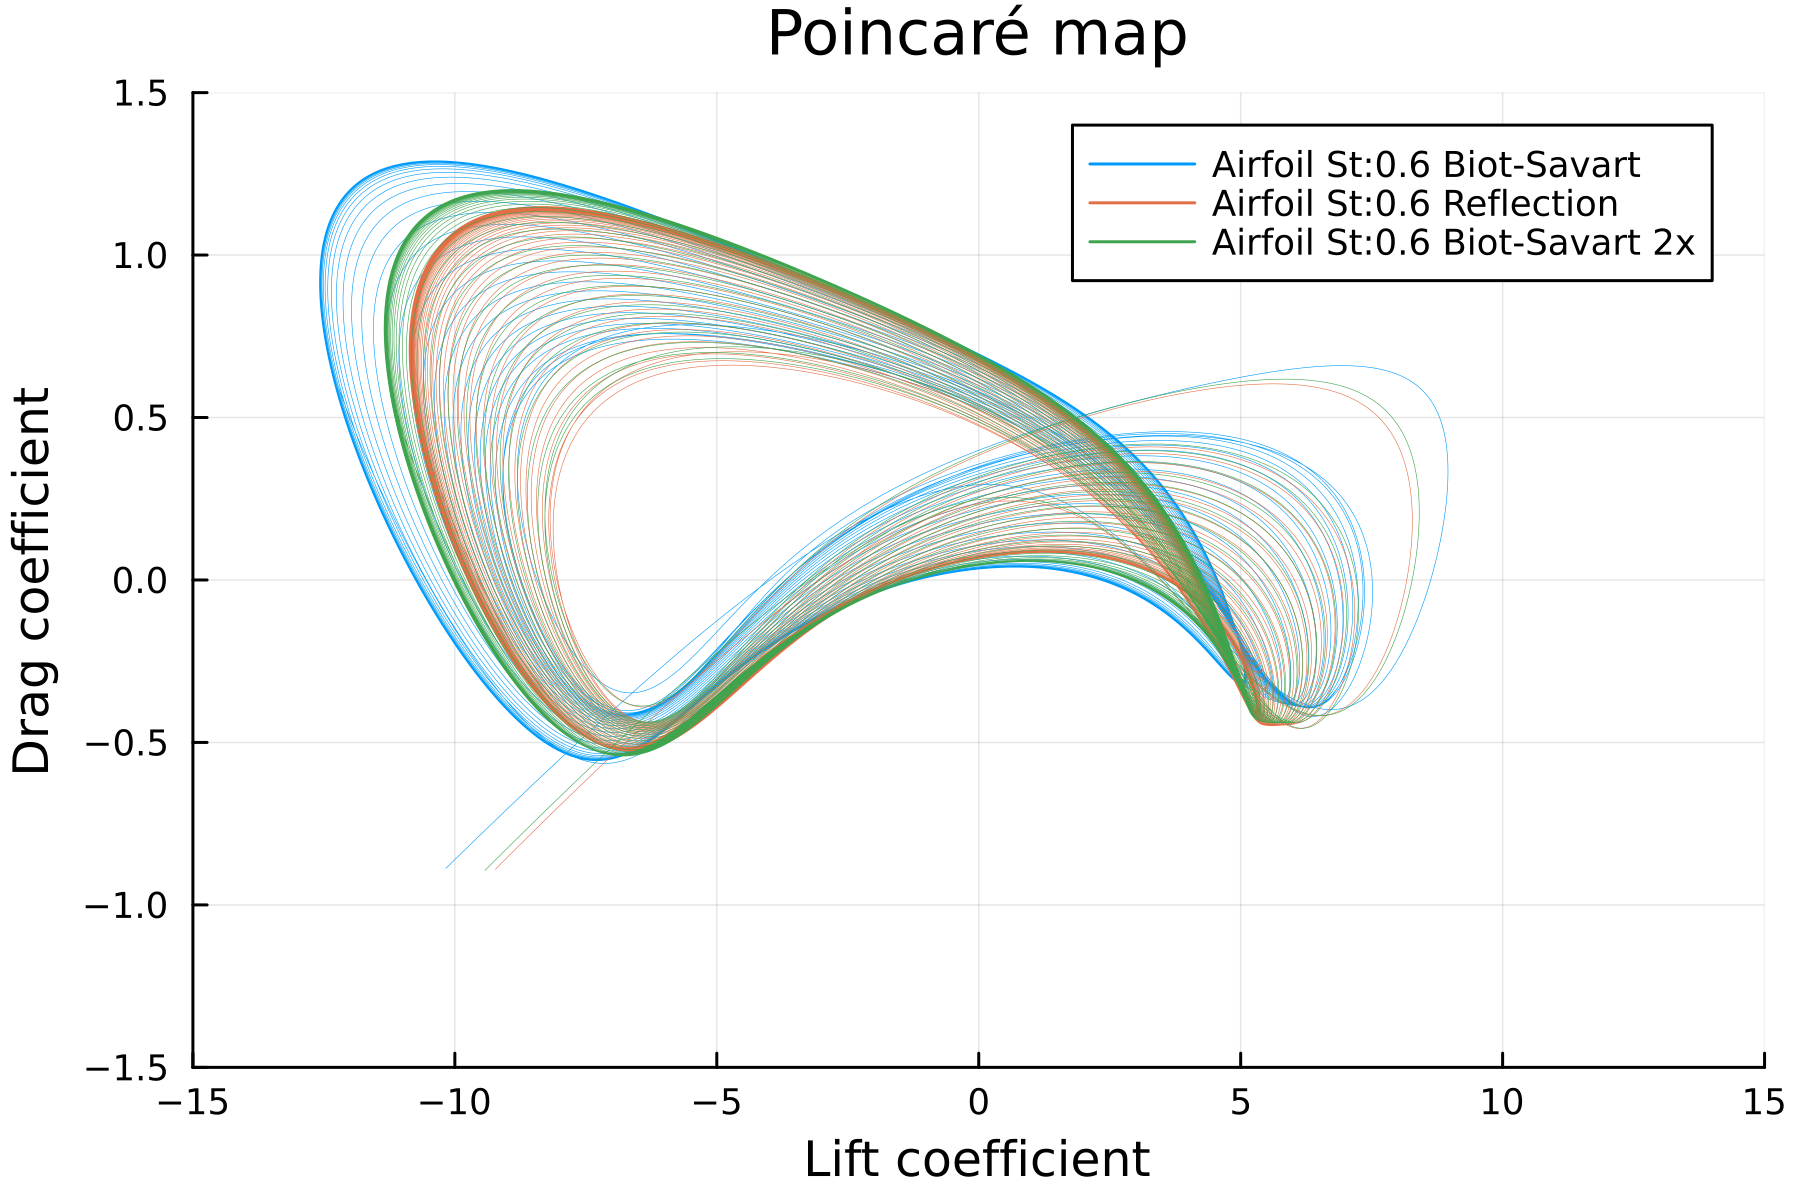
\includegraphics[trim={0 0 0 0},clip,width=\textwidth]{tex/fig/poincare_deflected_wake.png}
    \end{subfigure}
    \caption{(left) Mean lift force acting on the airfoil at $Re=100$, for a range of Strouhal numbers for the \emph{Biot-Savart} and the reflective boundary condition  and (right) \emph{Poincar\'e} map of the lift and drag coefficients for $St=0.6$}
    \label{fig:deflected_wake_2}
\end{figure}

Without accurately accounting for this wake history by cutting the wake, this deflection is poorly captured, and the airfoil does not produce the typical large mean lift force associated with deflected wakes, see Fig.~\ref{fig:deflected_wake_2}. This high lift coefficient is generated from the high-velocity jets formed at the trailing edge of the airfoil (clearly observable on the right panels of Fig.\ref{fig:deflected_wake}), which are much weaker with our \emph{Biot-Savart} boundary conditions on the small domain compared to classical reflective boundary conditions on the large domain or the larger \emph{Biot-Savart} domain. While the small \emph{Biot-Savart} domain fails to accurately capture the wake effects, doubling the domain size, while still using the \emph{Biot-Savart} boundary conditions allows us to almost exactly recover the mean lift coefficient of the large domain and the reflective boundary conditions, see Fig~\ref{fig:deflected_wake_2}$b$. \emph{Poincar\'e maps} provide an excellent tool to examine the convergence of periodic orbits of dynamic systems. Fig.~\ref{fig:deflected_wake_2}$b$ shows such a map for the lift and drag coefficient of the heaving airfoil at $St=0.6$. The asymmetry in the lift, resulting in a net mean lift coefficient, is clearly observed for the larger domains (for both boundary conditions), while the small \emph{Biot-Savart} domain shows almost perfectly symmetric orbits. For simulation where wake history effects are important, our \emph{Biot-Savart} boundary condition required domains where this wake is allowed to be developed to accurately capture the resulting wake asymmetry and the large mean lift coefficients. 

While this is a limitation of our method, at least in terms of domain size, this flow is an artifact of 2D simulations and does not occur in actual flows. Indeed, experiments on finite foils have shown that these high-lift deflected jets cannot form for finite wings, see \cite{Calderon2014OnWings, Godoy-DianaTransitionFoil}.

 
\section{Conclusion}


In this manuscript, we presented a novel boundary condition formulation for the incompressible Navier-Stokes equations. The methods rely on a \emph{Biot-Savart} integral of the vorticity inside the domain to set the velocity boundary conditions on the domain's face. We couple these boundary conditions with an explicit projection scheme to solve the coupled momentum and continuity equation in their primitive variables form. Leveraging the fast decaying properties of the \emph{Biot-Savart} kernel, we use a multigrid algorithm to reduce the number of operations required to update the boundary nodes from $N^2$ to $N\log N$ and show that the error introduced by this multigrid approach is bounded and can be estimated based on the dimension of the problem. We demonstrate that when a body is immersed in a domain using these boundary conditions, a coupling between the immersed body and the domain's boundary is introduced. We show that because this coupling only results in a weakly non-linear pressure Poisson equation, a simple differed correction approach can be used to solve the coupled Projection-\emph{Biot-Savart} step, allowing the use of standard Poisson solver.

With different examples of confined vorticity application, we show that the novel boundary conditions allow for a significant reduction in the size of the computational domain without any loss in accuracy. For accelerated flows, we show that the pressure field is unaffected by our boundaries and the resulting pressure force are free of any blockage effects.

Surpisingly, for vortex street applications, the method demonstrates its robustness and perfectly captures the drag forces and vortex shedding frequencies generated by a 2D circular cylinder at $Re=200$, even with minimal domain sizes ($5D\times3D$). Lastly, we show that the method is limited when strong wake history influences the flow in the near wake. For a high-amplitude, high-Strouhal number heaving airfoil, we show that capturing the deflected wake of the flow requires significantly larger domain (with our \emph{Biot-Savart} boundary conditions) and that the computational advantage is somewhat lost.

We believe that for confined vorticity application, such as accelerated bodies in the initial phase ($t^*<10$), when the vorticity is still confined to the body, this method is promising.

% \section*{Acknowledgments}
% This was supported in part by......


%Bibliography
\bibliographystyle{unsrt}  
\bibliography{references}  


\end{document}